\documentclass[12pt,spanish]{thesis}
\usepackage[latin1]{inputenc}
\usepackage[spanish]{babel}
\usepackage{amsmath}

%Interlineado
\usepackage{setspace}
\setstretch{1.5}

\usepackage{textcomp}
\usepackage{times}
\usepackage{amssymb}
\usepackage{float}
\usepackage{color}
\usepackage{graphicx}
\usepackage{eso-pic}
\usepackage{multicol}
\usepackage{enumerate}
\usepackage{url}
\usepackage{soul}
\usepackage{fancyhdr}
\usepackage{lscape}
\usepackage{pdfpages}
\usepackage{hyperref}
\usepackage{listings}

%Margenes
\usepackage[top=3cm,bottom=3cm,left=4.2cm,right=3cm]{geometry}
\pagestyle{empty} 
\frenchspacing
\fancyhead[L]{}
\fancyhead[C]{}
\fancyhead[R]{}
\fancyfoot[R]{\thepage}
\fancyfoot[C]{}


%Fin Preambulo
%%%%%%%%%%%%%%%%%%%%%%%%%%%%%%%%%%%%%%%%%%%%%%%%%%%%%

\begin{document}
\thispagestyle{empty}

\begin{center}
\linespread{1.15}
\textbf{\large{UNIVERSIDAD T�CNICA FEDERICO SANTA MAR�A\\}
\normalsize{DEPARTAMENTO DE ELECTR�NICA\\VALPARA�SO - CHILE\\}}

\vspace{0.5cm}
\begin{figure}[H]
\centering
  
\includegraphics[width=5.85cm]{figuras/usmLogo.png}
\end{figure}
\vspace{0.5cm}

\linespread{1}\hangindent=0cm
\textbf{\Large ``Desarrollo de un dispositivo electr�nico para monitoreo remoto de pacientes''\\}
\vspace{3cm}
\hangindent=0cm\large \textbf{Felipe Cordero Vera}\\
\vspace{0.5cm}
\hangindent=0cm\normalsize \textbf{MEMORIA DE TITULACI�N PARA OPTAR AL T�TULO DE INGENIERO CIVIL ELECTR�NICO}\\
\vspace{1cm}
\hangindent=0cm\normalsize \textbf{PROFESOR GUIA: \hspace{2cm} Marcos Z��iga B.}\\
\vspace{0.5cm}
\hangindent=0cm\normalsize \textbf{PROFESOR CORREFERENTE: \hspace{2cm} Daniel Erraz L.}\\

\end{center}

\thispagestyle{empty}
\newpage
\pagestyle{fancy}
\renewcommand\headrulewidth{0pt}
\renewcommand{\listfigurename}{�ndice de figuras}
\renewcommand{\listtablename}{�ndice de tablas}

%Numeros romanos al pie de pagina, secciones sin numero.
\pagenumbering{roman}
\section*{Agradecimientos}
Terminado este trabajo de t�tulo se cierra un largo ciclo Universitario, en el que he vivido distintas
experiencias que me han hecho crecer como profesional y como persona.

Quisiera agradecer a todos
los participantes de esta etapa, que son bastantes, demasiados para que pueda mencionarlos a todos,
sin embargo no quiero que olviden lo mucho que significaron para m� en este proceso. 

Quiero agradecer a mi padre y a mi madre, quienes han estado siempre para ayudarme, me han
apoyado en mis decisiones y han dado todo por m�. Su fe en m� y su apoyo continuo me dieron las
fuerzas para enfrentar los desaf�os que se me presentaban.
A mi hermana, mi familia, mis amigos, mis compa�eros, gracias por su preocupaci�n, su ayuda,
su apoyo y sus ense�anzas.

\newpage
\section*{Resumen}
Este trabajo consistir� en el desarrollo de un dispositivo electr�nico para monitoreo remoto de pacientes con distintos sensores que sea usable, de bajo costo y aut�nomo con env�o de informaci�n mediante conexi�n bluetooth de bajo consumo. 
Para lograr lo anterior se comenzar� buscando alternativas existentes en el mercado y se desarrollar� un prototipo funcional para evaluar a partir de las componentes disponibles. Finalmente a partir del prototipo funcional se realizar� el dise�o del esquem�tico y el circuito impreso en el programa EagleCAD para ser enviado a producci�n.\par
Es importante destacar que para el dise�o del dispositivo electr�nico se espera mantener el est�ndar de tecnolog�as que existen en la actualidad como el uso de bater�a interna recargable y que sea de f�cil uso para el usuario.
\newpage

%\section*{Abstract}

%\newpage

\section*{Glosario}

\begin{tabular}{lcp{10.5cm}}
Esquem�tico &:& Es una representaci�n pict�rica de un circuito electr�nico. Muestra las diferentes componentes del circuito de manera simple y las conexiones de alimentaci�n y se�ales entre distintos dispositivos.\\
PCB &:& Printed Circuit Board, El circuito impreso se utiliza para conectar el�ctricamente a trav�s de las pistas conductoras, y sostener mec�nicamente, por medio de la base, un conjunto de componentes electr�nicos.\\
Hardware &:& Partes f�sicas tangibles de un sistema inform�tico.\\
Software &:& Aplicaciones o programas que funcionan en un sistema inform�tico.\\
Firmware &:& Programa inform�tico que establece la l�gica de mas bajo nivel que controla los circuitos electr�nicos.\\
Bootloader &:& Es un programa que no tiene la totalidad de las funcionalidades para operar un sistema y est� dise�ado para preparar todo lo que necesita el firmware para ejecutarse.\\
IIH &:& Infecci�n Intra-Hospitalaria
\end{tabular}

%%%%%%%%%%%%%%%%%%
%\begin{tabular}{lcp{10.5cm}}
%Rel�&:& Interruptor controlado por un circuito el�ctrico en el que, por medio de una bobina y un electroim�n, se acciona un juego de uno o %varios contactos que permiten abrir o cerrar otros circuitos el�ctricos independientes.\\
%\end{tabular}
%%%%%%%%%%%%%%%%%%

%Se sigue con numeros arabes al pie de pagina
\pagenumbering{arabic}
\tableofcontents
\newpage
\listoffigures
\newpage
\listoftables

\newpage
\chapter{Introducci�n}\label{chap1}
\section{Memorias multidisciplinaria}
La UTFSM ha manifestado, a trav�s de sus planes de desarrollo y ejes estrat�gicos, la importancia de la formaci�n de los estudiantes en competencias transversales, el fomento de la innovaci�n, el emprendimiento y la vinculaci�n con la industria. Es por esto que surge en la UTFSM el proyecto de Memorias Multidisciplinarias que propone impulsar el desarrollo de una nueva industria tecnol�gica a trav�s de un programa de formaci�n para la creaci�n sistem�tica y sustentable de productos de innovaci�n y emprendimientos ligados a tecnolog�a.

Este proyecto de Memorias Multidisciplinarias se desarrolla a trav�s de la proposici�n de un desaf�o el cual fue otorgado por el subgerente comercial de la empresa Sistemas Expertos, Jos� Luis Araya. Sistemas Expertos e Ingenier�a de Software (SEIS) es una empresa especialista con 10 a�os de experiencia en el desarrollo e implementaci�n de soluciones tecnol�gicas para el �rea de la salud.

El desaf�o propuesto consiste en �C�mo podemos incorporar a bajo costo telemedicina a la salud p�blica, considerando restricciones econ�micas y geogr�ficas?. Para esto hubo una conformaci�n de un equipo multidisciplinario quienes desarrollaron durante un a�o, un plan de negocio, pruebas de concepto y prototipado de la soluci�n con lo cual se pretende formar un emprendimiento.
A ra�z de las necesidades del desaf�o propuesto por la empresa Sistemas Expertos, se hace necesaria la incorporaci�n de conocimientos en el �mbito t�cnico a nivel Hardware, Software, Telecomunicaciones, administraci�n de proyectos, marketing, an�lisis de consumidor, prototipado y posterior encapsulamiento de la soluci�n. Es por lo anterior que el equipo est� compuesto por cuatro integrantes.
\subsection{Felipe Cordero}
Estudiante de �ltimo a�o de la carrera Ingenier�a Civil Electr�nica con Menci�n en Computadores. Ha trabajado en empresas de desarrollo de hardware embebido, tiene un gran inter�s por crear un emprendimiento y seguir el camino de desarrollo de hardware y software. Su inter�s en el desaf�o radica en participar de un proyecto que posee todas las fases de desarrollo de hardware con un cliente desde cero. Al estar relacionado con el �rea de salud y conectividad  permite aportar directamente a mejorar el sistema de salud p�blica en Chile. 
\subsection{Vanessa Mu�oz}
Estudiante 5to a�o de Ingenier�a Comercial, 25 a�os. Colaborado en actividades dentro de la universidad como Preusm y actualmente trabajando por tercer a�o en la Feria de Empresas y Trabajo USM desempe��ndose como Coordinadora General. La principal motivaci�n por escoger este desaf�o es poder intervenir y mejorar alg�n �rea del sistema de la salud p�blica Chilena, dado que se ha podido presenciar la ineficiencia del servicio en distintas ocasiones. 
Decide abandonar el grupo por no cumplir los objetivos buscados para su trabajo de tesis.
\subsection{Patricio Rodr�guez}
Estudiante de �ltimo a�o en la carrera de Ingenier�a Civil Telem�tica. Ha contribuido en distintos proyectos relacionados a procesamiento de imagen, an�lisis de redes, simulaci�n, programaci�n, entre otros. Se destaca por su gran motivaci�n y tenacidad a la hora de desempe�ar sus tareas, aportando al trabajo en equipo y facilitando la resoluci�n de tareas. Su inter�s en el desaf�o recae en la necesidad de conectividad que este conlleva, adem�s de estar ligado al �rea de la Salud. �rea de especial inter�s considerando la distancia profesional que se puede alcanzar estudiando una carrera de Ingenier�a.
\subsection{Sebasti�n Castillo}
Estudiante de �ltimo a�o en la carrera de Ingenier�a en Dise�o de Productos. Participado en actividades relacionadas al voluntariado, desarrollo de proyectos tecnol�gicos y conservaci�n de la naturaleza. Se perfila como un profesional vers�til, comprometido y que considera el trabajo multidisciplinario como fundamental en el desarrollo de soluciones para el mundo actual. El inter�s en este proyecto se debe a la posibilidad de poder impactar positivamente en la vida de gente con necesidades reales y mejorar, en cierta medida, su calidad de vida a trav�s de la ingenier�a, que muchas veces olvida el rol social que puede ejercer
\section{An�lisis del desaf�o}
La empresa Sistemas Expertos ha planteado el desaf�o: �C�mo podemos incorporar a bajo costo telemedicina a la salud p�blica, considerando restricciones econ�micas y geogr�ficas?. 
En donde se da cuenta de la necesidad actual de aplicar las tecnolog�as existentes en el �mbito de salud, permitiendo de esta forma mejorar la atenci�n. Para conseguir este objetivo se espera el desarrollo de un dispositivo electr�nico con capacidad de toma de datos y env�o de los mismos. As�, se pueden identificar distintas aristas a considerar, como lo son: Tipo de enfermedades y pacientes a cubrir, tipo de sensores a emplear, tipo de tecnolog�a de comunicaci�n, nivel de interacci�n con el usuario, entre otros.

Con esto en mente, se debe tomar una decisi�n con respecto a las enfermedades a medir ya que esto est� ligado �ntimamente a los sensores a utilizar pudi�ndose encontrar entre ellos: electrocardiograma, saturometro, medidor de presi�n, term�metro, entre otros.

Adem�s de lo anterior, para realizar la comunicaci�n de estos datos de forma remota se contemplan distintas alternativas, entre las que se considera utilizar la infraestructura ya presente e implementada en el pa�s, como lo son las antenas celulares conectadas directamente con el dispositivo y tambi�n utilizar conexi�n a internet con un intermediario como un smartphone mediante una conexi�n bluetooth.

Por �ltimo, respecto al nivel de interacci�n con el usuario, la empresa ha dejado expresa su necesidad de simplicidad en este desarrollo, descartando cualquier interfaz o comunicaci�n directa entre el usuario final y el dispositivo. Si bien dependiendo de la tecnolog�a a emplear esta sugerencia puede cambiar, en una primera instancia se mantiene esta l�nea de pensamiento en torno al desarrollo completo, intentando as� mantener la sencillez en las distintas partes del dispositivo. Permitiendo de este modo reducir los datos a manipular, las interfaces a desarrollar y el riesgo de un mal uso por parte de los usuarios.\\


\section{Estado del Arte}
En el marco del desarrollo del desaf�o de Sistemas Expertos, se plante� generar un dispositivo de monitoreo a distancia de pacientes. Para esto se comenz� a estudiar aspectos relacionados con la Telemedicina y sus implicancias en el avance del monitoreo Remoto de Paciente (RPM, por sus siglas en ingl�s). La Telemedicina es, en principio, la tecnolog�a que permite entregar cuidados m�dicos a trav�s de la infraestructura de las telecomunicaciones, permitiendo a los m�dicos diagnosticar o evaluar enfermedades sin la necesidad de un control presencial.
Para poder comprender en qu� se encuentra la realidad nacional y latinoamericana es de suma importancia revisar algunos casos d�nde se apliquen dispositivos de telemedicina bajo la modalidad de monitorear y digitalizar la informaci�n, considerando que el objetivo del proyecto se limita a esas dos acciones.

\subsection{ViSi Mobile\textregistered}
ViSi Mobile\textregistered\;\cite{visi}, si bien se utiliza en el cuerpo, es una estaci�n que procesa los datos de otros sensores que van colocados en el cuerpo y que a su vez se conectan al m�dulo central de procesamiento como se puede observar en la imagen 1 lo que es necesario categorizarlo como un producto modular. Los sensores se encargan de medir pulso, respiraci�n, SpO2, presi�n sangu�nea continua no invasiva y temperatura de la piel. El principal objetivo es permitir monitorear al paciente de forma  continua dentro del hospital, sin intervenir de manera negativa en el flujo de trabajo que all� existe (ViSi Mobile\textregistered\; System, s. f.). ViSi Mobile\textregistered\; se encarga de recopilar los datos que cada sensor pueda otorgar para luego enviarlos de manera simult�nea a un smartphone, una plataforma online de monitoreo y adem�s directo a la estaci�n de trabajo del m�dico a cargo, permitiendo as� una atenci�n eficiente.

\begin{figure}[H]
\centering
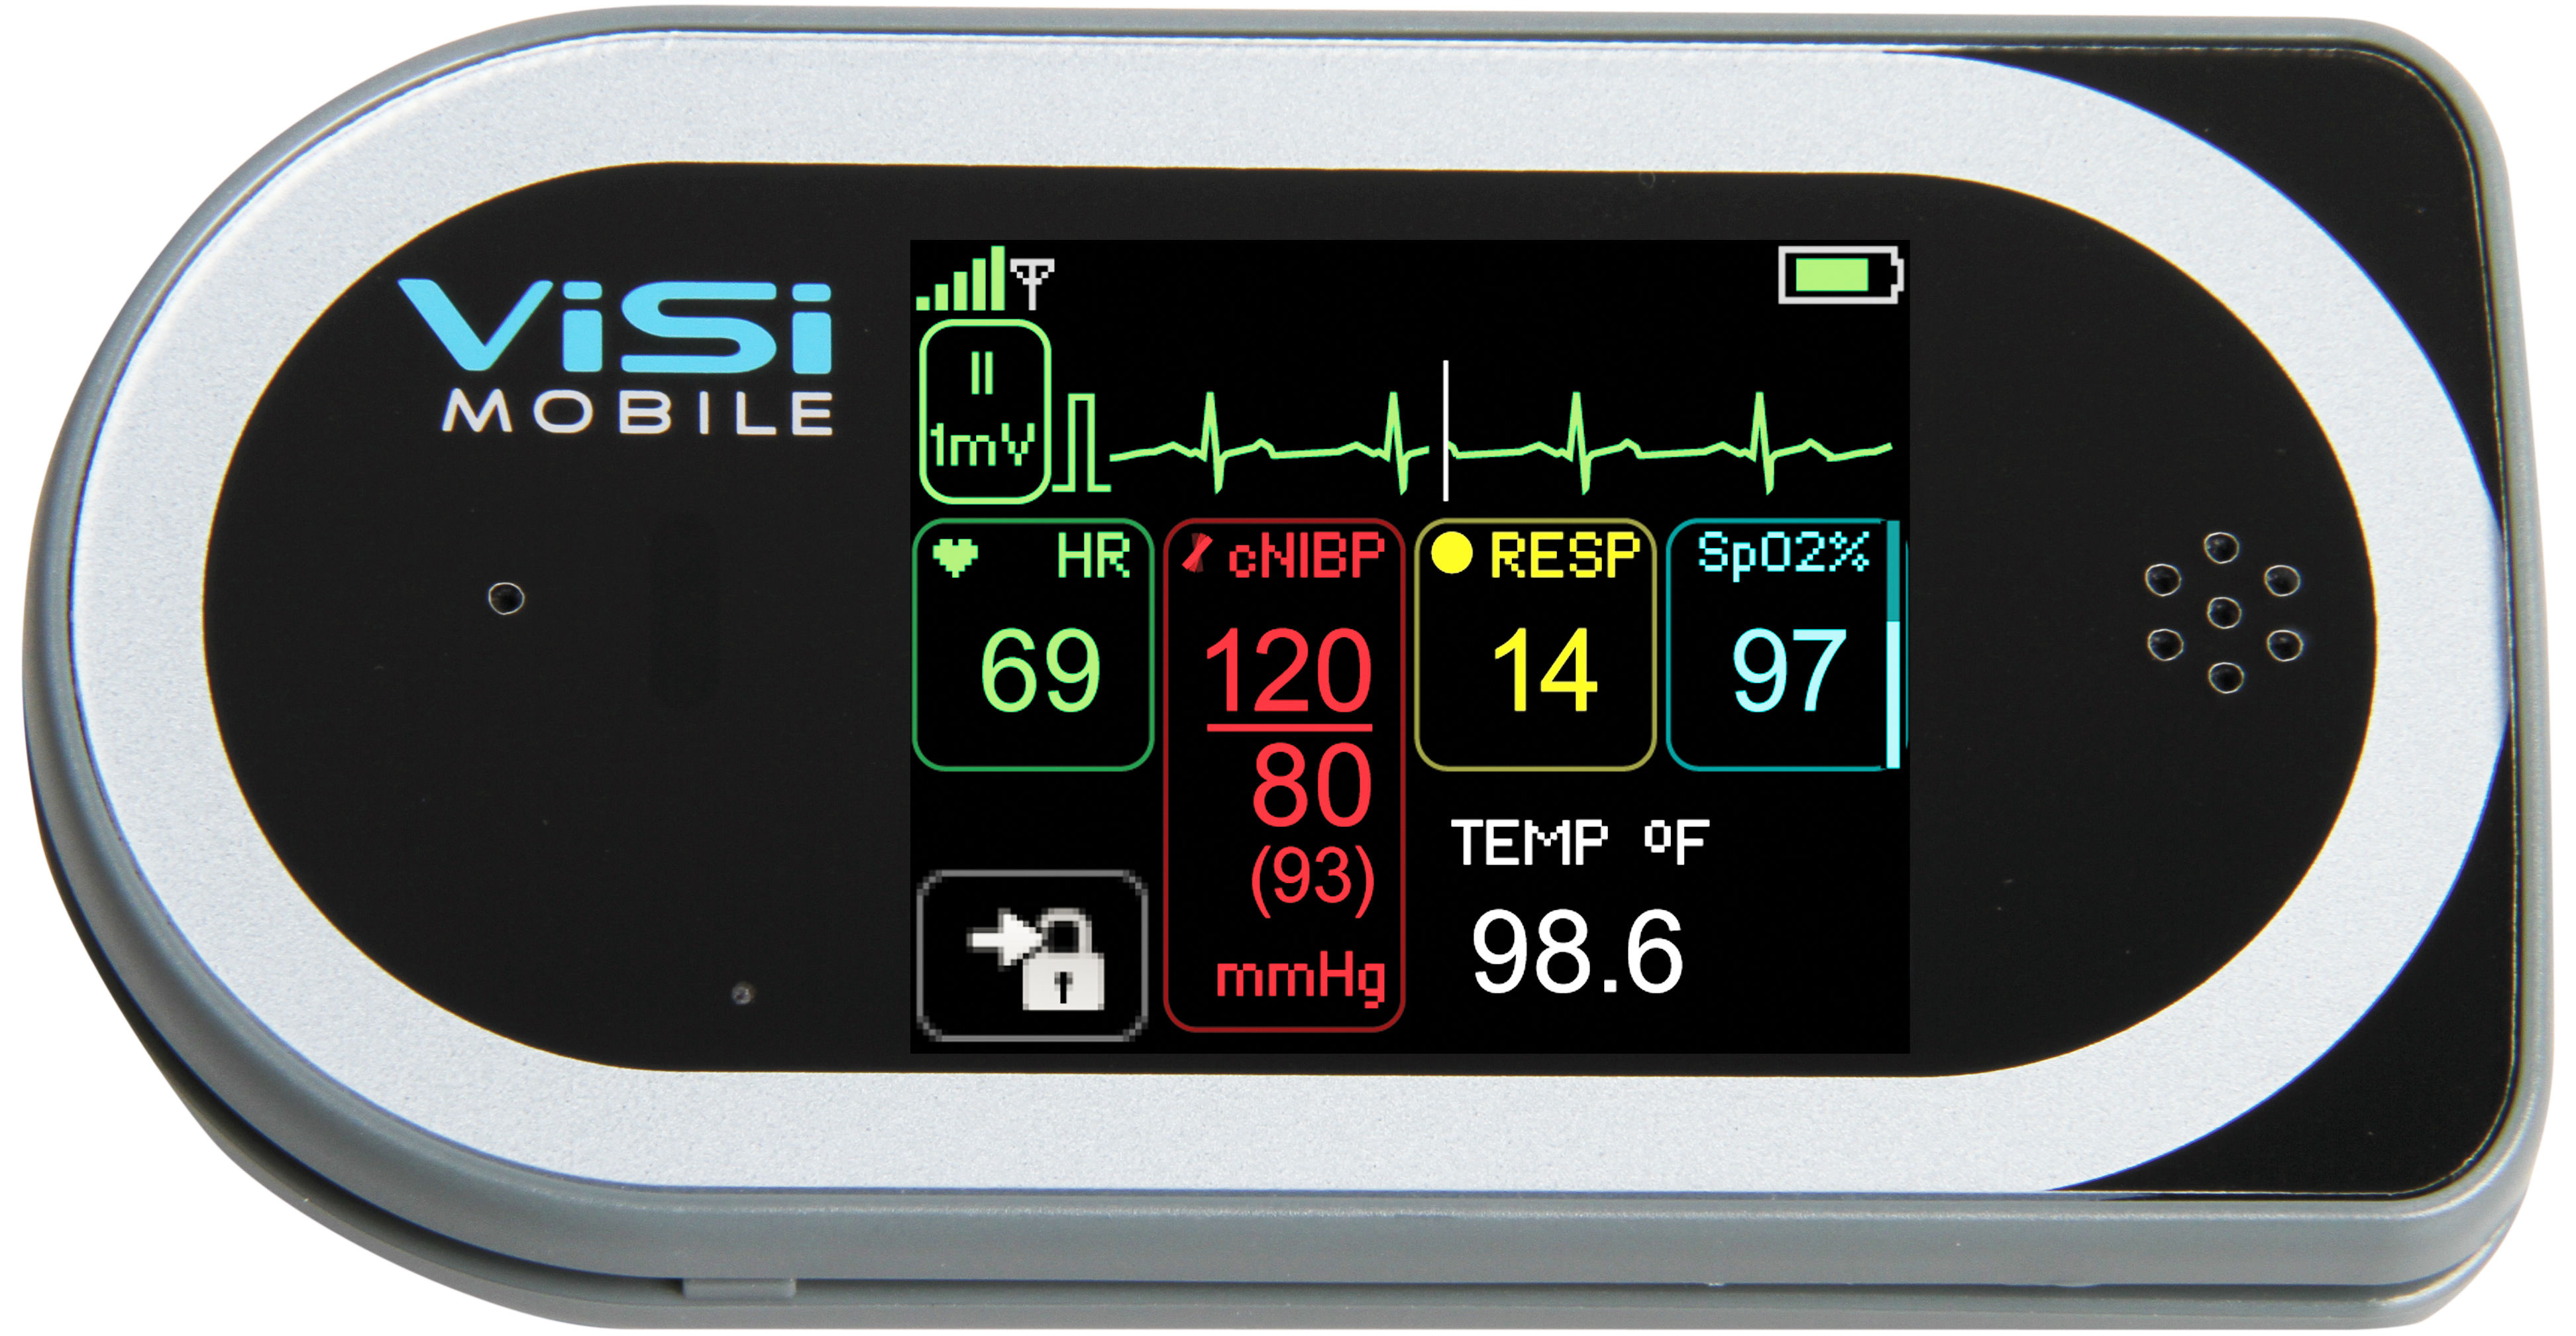
\includegraphics[scale=0.3]{figura/estadoarte/visi/visi.jpg}
\caption{Interfaz de usuario ViSi Mobile\textregistered}
\label{visi1}
\end{figure}

Se puede observar en la figura \ref{visi1} la interfaz que puede ver el paciente al utilizar el dispositivo.

\begin{figure}[H]
\centering
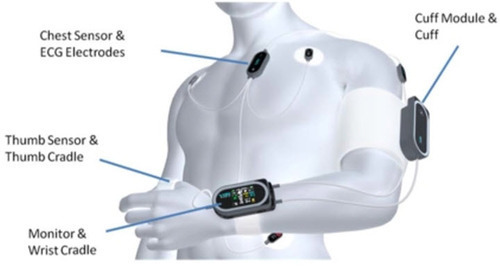
\includegraphics[scale=0.7]{figura/estadoarte/visi/wear.jpg}
\caption{Modo de uso ViSi Mobile\textregistered}
\label{visi2}
\end{figure}

En la imagen de la figura \ref{visi2} se puede observar los sensores conectados al cuerpo que convergen al dispositivo que toma las se�ales.

\subsection{Qardiocore}

QardioCore\cite{qardio} es un monitor de electrocardiograma inal�mbrico dise�ado para mejorar la detecci�n y manejo de las condiciones card�acas. Seis sensores se encargan de grabar y analizar sobre 20 millones de puntos de datos durante todo el d�a junto con otros signos vitales. Este dispositivo est� orientado a personas con alto nivel de riesgo card�aco causado por predisposici�n familiar, historial de ataques al coraz�n, presi�n alta, colesterol alto, diabetes o exceso de peso. Monitorea de forma precisa y continua la salud del coraz�n. El dispositivo graba datos de ECG, pulso, variaci�n de pulso, temperatura corporal, ritmo respiratorio y niveles de estr�s. A diferencia de los ECG tradicionales, QardioCore no utiliza gel ni cables para monitorear y funciona entre -20�C y 60�C. Adicionalmente es resistente al agua y su bater�a dura alrededor de un d�a.\\

\begin{figure}[H]
\centering
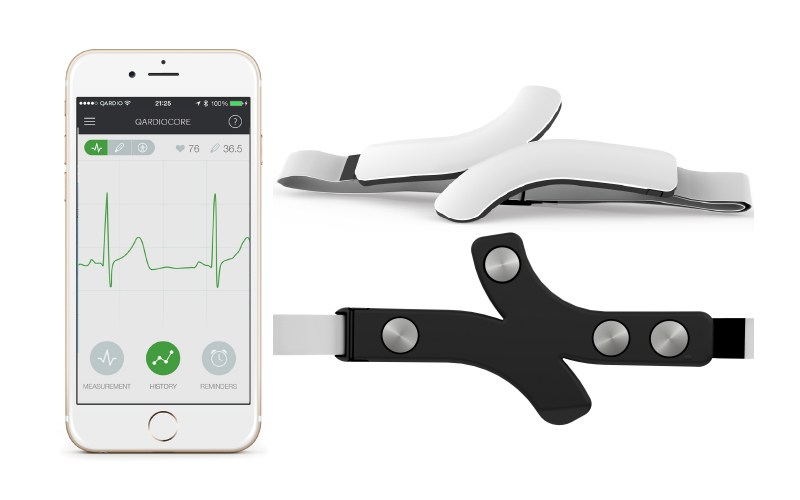
\includegraphics[scale=0.5]{figura/estadoarte/qardio/qardio.jpg}
\caption{Qardiocore multisensor}
\label{qardio1}
\end{figure}

Se puede observar el dispositivo Qardiocore en la figura \ref{qardio1} que se conecta a un smartphone para mostrar los datos que se est�n tomando.
Adem�s como se muestra en la figura \ref{qardio2} es de simple uso, funciona como un cintur�n en el pecho del paciente.

\begin{figure}[H]
\centering
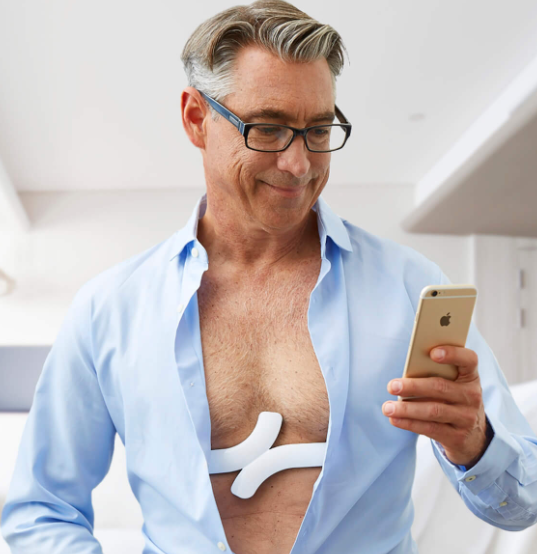
\includegraphics[scale=0.5]{figura/estadoarte/qardio/wear.png}
\caption{Modo de uso Qardiocore}
\label{qardio2}
\end{figure}

\subsection{Nuubo}

Nuubo\cite{nuubo} proporciona una nueva perspectiva en la monitorizaci�n cardiol�gica remota e inal�mbrica. La plataforma de Nuubo, nECG platform, permite la captura del ECG din�mico a trav�s de un innovador sistema que est� basado en textiles biom�dicos de nueva generaci�n, y es rentable, remoto, continuo y no invasivo. Adem�s, puede ser utilizado simult�neamente con uno o varios pacientes.
La tecnolog�a de electrodos textiles desarrollada por Nuubo simplifica enormemente los inc�modos procedimientos tradicionales de conexi�n de electrodos, reduci�ndolos al sencillo acto de vestir la camiseta nECG SHIRT que se muestra en la figura \ref{shirt}.
 
\begin{figure}[H]
\centering
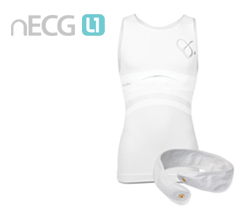
\includegraphics[scale=0.6]{figura/estadoarte/nuubo/shirt.png}
\caption{nECG Shirt}
\label{shirt}
\end{figure}

El tejido el�stico se adapta a los movimientos del paciente, quien puede realizar su actividad f�sica diaria sin estar limitado por cables y sin necesidad de depender de personal m�dico especializado. Estas caracter�sticas junto con la informaci�n de contexto, la actividad f�sica del paciente y su posici�n/postura, permite el desarrollo de un nuevo rango de soluciones y casos de uso. 

\begin{figure}[H]
\centering
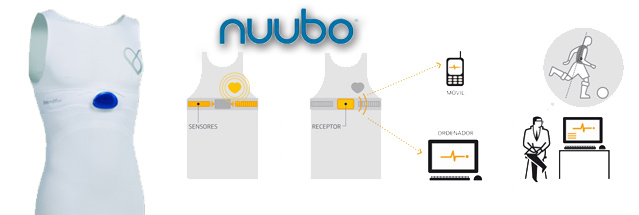
\includegraphics[scale=0.7]{figura/estadoarte/nuubo/nuubo.png}
\caption{Sistema Nuubo}
\label{nuubo}
\end{figure}

Como se puede observar en la figura \ref{nuubo} la polera toma los datos que son enviados a un dispositivo movil o un computador para que sea visto por el doctor de manera remota.

\newpage
% ---------------------------------------------------------------------------------------
\chapter{Alternativas de desarrollo}\label{chap2}
En el presente cap�tulo se ahondar� en las distintas alternativas de dise�o que existen para el prototipo con los distintos sensores requeridos, adem�s de establecer la comunicaci�n y el env�o de la informaci�n tomada del paciente. Las etapas para el desarrollo del prototipo constan de: Elecci�n de sistema de procesamiento o unidad central, sensores a utilizar y forma de comunicaci�n inal�mbrica.
\section{Plataforma de desarrollo}\label{proce}
Al fabricar un prototipo, el desarrollador debe construir el hardware sobre el cual correr� el software del producto que ha dise�ado, por lo que debe tomar componentes de diversos proveedores, integrarlos y hacerlos funcionar como un conjunto. Por esa raz�n se populariz� el uso de plataformas de desarrollo electr�nico.  \\
Por lo general, estas son placas que integran microcontroladores, circuitos y componentes electr�nicos que le proporcionan diversas capacidades b�sicas y a partir de esto se puede evaluar la compatibilidad del dise�o tanto en hardware como en software antes de enviar a fabricar el producto final. 

\newpage
\subsection{Arduino}
Arduino es una plataforma de desarrollo de bajo costo que permite crear proyectos de base tecnol�gica de forma sencilla y barata, que consta de entradas an�logas, entradas y salidas digitales, PWM, comunicaci�n serial, etc. 

Uno de los beneficios de Arduino es que provee m�dulos de desarrollo de bajo costo para trabajar con integrados y estudiar su funcionamiento y prototipado.
Arduino trabaja con una gran variedad microcontroladores AVR que diferencia por modelos dependiendo de las necesidades de proyecto, motivo por el cual var�a en precio. 

En primera instancia se puede trabajar con un modelo Arduino UNO que es de bajo costo y permite leer se�ales an�logas y traducirlas en su conversor an�logo-digital y dependiendo de las necesidades se puede conseguir otro modelo como Arduino Mega que ofrece mayores prestaciones. 
\subsection{Raspberry}
Raspberry es una computadora de placa reducida (SBC por sus siglas en ingl�s) de bajo costo, con el objetivo de estimular la ense�anza de ciencias de la computaci�n, no obstante, es de propiedad registrada para poder mantener el control de la 8 plataforma y no se generan excesivas variantes como es el caso de Arduino. El software que usa es open source, aunque es capaz de ejecutar incluso una versi�n de Windows 10. Por lo mismo su capacidad de procesar se�ales es mayor y permite ejecutar proyectos m�s complejos. No se define si es que pueden o no ser usadas en desarrollos comerciales.

\newpage
\subsection{Beaglebone}
Beaglebone black es la �ltima iteraci�n de la serie Beaglebone y su versi�n peque�a. Esencialmente es similar a Raspberry, diferenci�ndose en cosas como la capacidad para iniciarse sin la necesidad de instalar ning�n sistema operativo ya que tiene memoria integrada, no as� Raspberry. Adicionalmente cuenta con una cantidad de entradas sustancialmente mayor, por lo que permite hasta el doble de conexiones que su competencia directa. Como si es no fuera suficiente, la arquitectura del procesador que incluye Beaglebone black permite que rinda hasta el doble de r�pido que su contraparte en Raspberry pi. \\
Al igual que su competencia, Beaglebone ofrece mucho mas procesamiento que el necesario por lo que se descarta como una opci�n para el desarrollo inicial del prototipo, de acuerdo a las necesidades que vayan surgiendo se puede considerar nuevamente como una opci�n.
\newpage
\section{Sensores}
Hablando con la contraparte de Sistemas Expertos se decidi�, a partir de la informaci�n que proveen ellos, que las enfermedades  mas comunes son las afecciones card�acas y tambi�n es necesario tener un control de la temperatura de los pacientes a la hora de leer sus signos vitales. \\
Por otra parte se propuso utilizar una IMU para detectar si alg�n paciente sufre una ca�da, este con el fin de emitir una alarma para llamar una ambulancia en caso de ser necesario.
\subsection{ECG}
Electrocardiograma o ECG es el proceso de registrar la actividad el�ctrica del coraz�n en un periodo de tiempo usando electrodos directamente en la piel.\\
Lo fundamental ser� buscar un circuito de desarrollo para realizar una prueba de concepto, en la cual se puedan tomar los datos y manejar.
\subsubsection{DFRobot Heart Rate Monitor Sensor}
El monitor de actividad cardiaca de la empresa DFRobot se usa para medir la actividad electrica del coraz�n con un integrado AD8232\cite{ad8232} que toma se�ales an�logas de los electrodos y utiliza amplificadores para tener una mejor lectura de los datos.\\
Utilizando un Arduino es posible leer los datos tomados de los electrodos y convertirlos a informaci�n digital que puede ser enviada por comunicaci�n serial.\\

\begin{figure}[H]
\centering
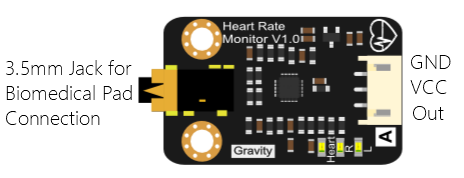
\includegraphics[scale=0.5]{figuras/sensor/ecg/ecg.png}
\caption{Placa de desarrollo ECG}
\label{ecg}
\end{figure}

Como se puede observar en la figura \ref{ecg} posee conexi�n simple para electrodos y salida an�loga, lo que permitir� una r�pida prueba de concepto para utilizar este integrado en el dise�o del dispositivo final. Adem�s este provee filtros que se van a estudiar mas adelante.


\subsubsection{ADS1298}
El integrado ADS1298 de la empresa Texas Instrument ofrece un ECG con 8 amplificadores programables de bajo ruido y 8 conversores An�logo-digital de alta resoluci�n.\\
Utilizado para instrumentaci�n medica y lectura tanto de ECG como EMG (Electromiograma) y EEG (Electroencefalograma).\\
El integrado ADS1298 es una buena opci�n para un desarrollo de ECG en el futuro de grado m�dico, pero es de un precio 10 veces mayor al dispositivo de DFRobot por lo que se va a descartar para el prototipo funcional.
\subsection{Temperatura}
Cuando se requiere realizar alguna medici�n a un paciente siempre es necesario conocer su temperatura corporal que sirve como informaci�n complementaria a los profesionales de la salud es por esto que se evaluar�n termistores que permitan la lectura de este dato.
\subsubsection{Lilypad Temperature Sensor}
Dentro de la tendencia del hardware abierto, uno de los proyectos m�s destacados es Lilypad Arduino, un conjunto de piezas electr�nicas que se pueden coser a los tejidos para darles interactividad con sensores, luces o sonidos.\\
Entre estos sensores tenemos un sensor de temperatura compuesto por un termistor MCP9700 el cual ofrece una resoluci�n de $\pm2^\circ C.$\\

\newpage
La particularidades que ofrece este sensor es ser de muy bajo costo y a su vez es impermeable por lo que permitir�a incorporarlo en el wearable de forma permanente sin da�ar la componente.

\begin{figure}[H]
\centering
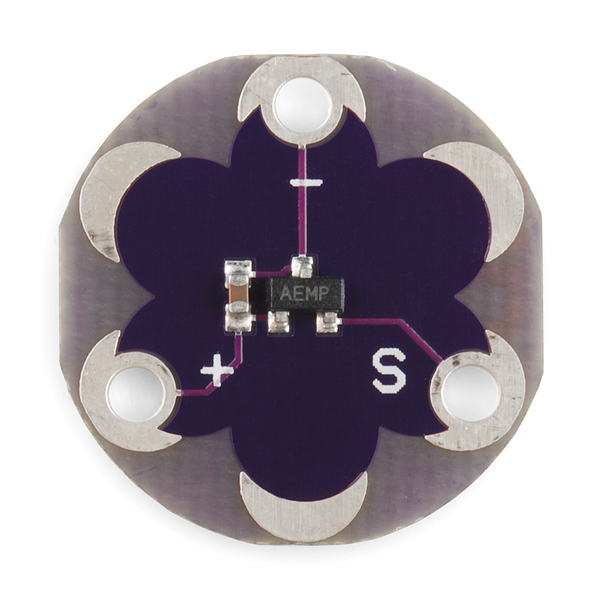
\includegraphics[scale=0.7]{figuras/sensor/t/lilypad.jpg}
\caption{Sensor de temperatura Lilypad}
\label{Lilypad}
\end{figure}

Como se puede observar en la figura \ref{Lilypad}, Lilypad ofrece una PCB impermeable con 3 terminales que permiten utilizar un hilo conductor para coser este a la ropa.

\subsubsection{DS18B20}
El sensor DS18B20\cite{temp} es un term�metro digital que ofrece una medida de 9 a 12 bits de resoluci�n. Se comunica mediante el bus 1-Wire (protocolo de comunicaci�n en serie dise�ado por Dallas Semiconductor el cual est� basado en un maestro y varios esclavos en una sola linea de datos) lo cual permitir�a, en caso de ser necesario, incorporar mas sensores para obtener una medida con mayor precisi�n. 
Este term�metro digital ofrece una resoluci�n de $\pm0.5^\circ C$ y a su vez ofrece un formato impermeable en forma cil�ndrica como se observa en la figura \ref{DS18B20}.

\begin{figure}[H]
\centering
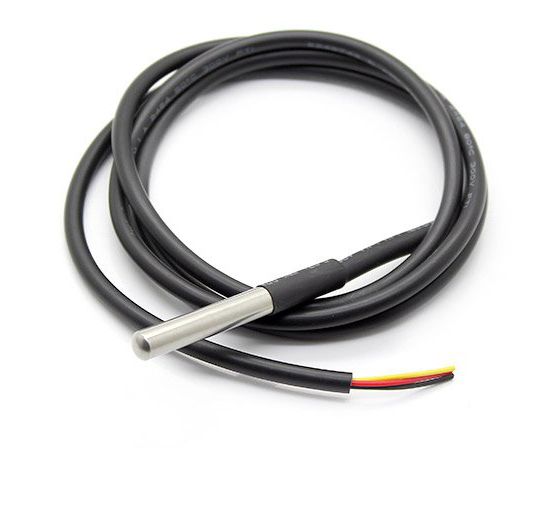
\includegraphics[scale=0.2]{figuras/sensor/t/ds18.jpg}
\caption{Sensor de temperatura DS18B20}
\label{DS18B20}
\end{figure}

\subsection{Ritmo Respiratorio}
Para medir el ritmo respiratorio, sensor que la contraparte pidi� estudiar utilizando una tela conductora, se consider� el uso de la tela conductiva MedTex, la cual entrega un valor de resistividad en ohms en su estado en reposo y este var�a dependiendo de su estiramiento.\\

\begin{figure}[H]
\centering
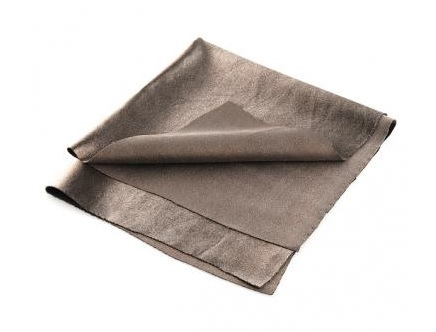
\includegraphics[scale=0.5]{figuras/tela/medtex.jpg}
\caption{Tela Conductiva MedTex}
\label{medtex}
\end{figure}

Para estudiar la factibilidad de la tela conductiva que se puede observar en la figura \ref{medtex} se cort� una tira de un tama�o $20x2 [cm]$ en estiramiento cero sobre una banda el�stica que luego fue cosida como cintur�n de pecho. Una vez colocada en cada extremo de la tela conductiva se coloc� un caim�n conectado a su vez a un multitester que permit�a visualizar variaciones de la resistividad de la tela a partir de su estiramiento. 

\newpage
\begin{table}[H]
\centering
\begin{tabular}{| c | c | c |}
\hline
\multicolumn{1}{|c|}{\textbf{Resistencia en reposo [$\Omega$]}}&
\multicolumn{1}{c|}{\textbf{Resistencia en estiramiento [$\Omega$]}}&
\multicolumn{1}{|c|}{\textbf{\% de variaci�n)}}\\ \hline
$4.8$  & $4.6$  & $0.1420$  \\ \hline
$4.7$  & $4.5$ & $0.1421$ \\ \hline
$4.8$ & $4.7$  & $0.0722$  \\ \hline
\end{tabular}
\caption{Valores resistencia Tela MedTex en Pectorales}
\label{tablatex1}
\end{table}

\begin{table}[H]
\centering
\begin{tabular}{| c | c | c |}
\hline
\multicolumn{1}{|c|}{\textbf{Resistencia en reposo [$\Omega$]}}&
\multicolumn{1}{c|}{\textbf{Resistencia en estiramiento [$\Omega$]}}&
\multicolumn{1}{|c|}{\textbf{\% de variaci�n)}}\\ \hline
$4.7$  & $4.6$  & $0.0699$  \\ \hline
$4.7$  & $4.6$ & $0.0699$ \\ \hline
$4.6$ & $4.5$  & $0.0723$  \\ \hline
\end{tabular}
\caption{Valores resistencia Tela MedTex en Plexo}
\label{tablatex2}
\end{table}

\begin{table}[H]
\centering
\begin{tabular}{| c | c | c |}
\hline
\multicolumn{1}{|c|}{\textbf{Resistencia en reposo [$\Omega$]}}&
\multicolumn{1}{c|}{\textbf{Resistencia en estiramiento [$\Omega$]}}&
\multicolumn{1}{|c|}{\textbf{\% de variaci�n)}}\\ \hline
$4.7$  & $4.6$  & $0.0699$  \\ \hline
$4.8$  & $4.7$ & $0.0722$ \\ \hline
$4.7$ & $4.5$  & $0.1421$  \\ \hline
\end{tabular}
\caption{Valores resistencia Tela MedTex en Estomago}
\label{tablatex3}
\end{table}

Se puede observar en las tablas \ref{tablatex1}, \ref{tablatex2} y \ref{tablatex3} las variaciones de resistencias no son constantes ni regulares, el mismo estiramiento a veces no produc�a la misma variaciones de resistencia. Adem�s por m�nimas variaciones en el movimiento tambi�n hab�an variaciones que arruinaban la medici�n, por lo que esta alternativa no ser�a viable para medir el ritmo respiratorio.

\subsection{Unidad de movimiento inercial (IMU)}
Una unidad de movimiento inercial o IMU (del ingl�s inertial measurement unit), es un dispositivo electr�nico que mide la aceleraci�n, inclinaci�n y las fuerzas gravitacionales, usando una combinaci�n de aceler�metros y giroscopios.
\subsubsection{MPU-9250}
El integrado MPU-9250 es un modulo multi-chip que consiste en 2 integrados en un empaquetado QFN. Este provee un giroscopio de 3 ejes y un aceler�metro de 3 ejes.
Este chip provee tres conversores an�logo-digital de 16 bits para digitalizar las salidas del giroscopio, aceler�metro y giroscopio de manera independiente.\\
Sparkfun provee una PCB de desarrollo para realizar pruebas como se muestra en la imagen \ref{imu1}.

\begin{figure}[H]
\centering
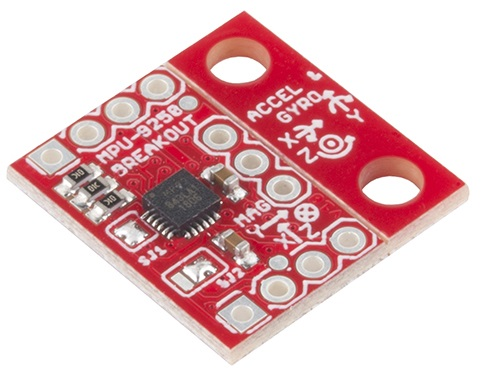
\includegraphics[scale=1.5]{figuras/sensor/imu/imu1.jpg}
\caption{IMU Sparkfun MPU-9250}
\label{imu1}
\end{figure}

Es importante destacar la orientaci�n indicada por el fabricante al momento de dise�ar el equipo electr�nico que son predefinidas como se puede ver en el caso de la figura \ref{imu1} en la cual se muestran los ejes X, Y y Z tanto para el aceler�metro como para el giroscopio. 
\newpage
Como se observa en la figura \ref{imu11} se muestra adem�s de los ejes de aceleraci�n tambi�n las coordenadas de navegaci�n (roll, pitch, yaw). 

\begin{figure}[H]
\centering
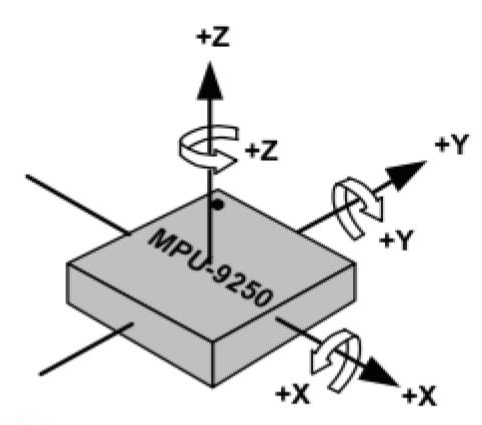
\includegraphics[scale=0.5]{figuras/sensor/imu/imu11.jpg}
\caption{Ejes IMU MPU-9250}
\label{imu11}
\end{figure}

\section{Comunicaci�n}
Para el proyecto se consideran distintas alternativas de conexi�n, las cuales deben seguir ciertos aspectos relevantes seg�n las especificaciones del dispositivo a implementar. 


\begin{enumerate}
	\item \textbf{Alta disponibilidad:}
	Se requiere que la tecnolog�a a emplear permita establecer conexiones a lo largo del tiempo, presentando pocas o de preferencia nulas desconexiones o incapacidades de conexi�n.
	\item \textbf{Gran cobertura:}
	Considerando la envergadura inicial del proyecto, Chile, es de vital importancia que la tecnolog�a a utilizar permita generar conexiones en la mayor parte del territorio nacional.
	\item \textbf{Bajo costo:}
	Dentro de los requerimientos del proyecto se encuentra el desarrollo e implementaci�n a bajo costo de la soluci�n final, por tanto la tecnolog�a de comunicaci�n a emplear debe seguir esta directriz para ser seleccionada.
	\item \textbf{Baja complejidad:}
	Considerando que el dispositivo en cuesti�n debiera ser lo m�s aut�nomo y sencillo de configurar, es relevante considerar tecnolog�as de comunicaci�n que no requieran de complejas operaciones para su uso e implementaci�n.
	\item \textbf{Escalabilidad:}
	Si bien es un aspecto dependiente de los anteriores requerimientos, es relevante considerarlo por separado como la medida que representa la capacidad de atender una gran cantidad de conexiones (usuarios en definitiva). 
\end{enumerate}

En base a lo anterior, se hace un an�lisis r�pido de diferentes alternativas que podr�an utilizarse en el proyecto:

\begin{enumerate}
\item \textbf{Antenas de RF:}\cite{RF}
Comunicaci�n generada en las bandas situadas entre los 3 kilohercios (KHz) y 300 Gigahercios (GHz). Esta tecnolog�a incluye distintas otras tecnolog�as como las redes celulares, pero en este apartado se especifica el uso de bandas no utilizadas por esta y otras tecnolog�as. Permitiendo una conexi�n directa de antena a antena a una frecuencia espec�fica a determinar.

\item \textbf{Comunicaci�n satelital:}\cite{satelite}
Comunicaci�n  por medio de ondas electromagn�ticas transmitidas gracias a la presencia en el espacio de sat�lites artificiales situados en �rbita alrededor de la Tierra. Dentro de esta tecnolog�a se pueden encontrar dos grandes clasificaciones: Sat�lites activos y Sat�lites pasivos, los cuales se diferencian por la amplificaci�n o de las se�ales antes de ser reenviadas a la Tierra, respectivamente.

\item \textbf{Redes Wi-Fi:}\cite{wifi}
Tambi�n llamada WLAN (Wireless lan, red inal�mbrica) o est�ndar IEEE 802.11, es una de las tecnolog�as de comunicaci�n inal�mbrica mediante ondas m�s utilizada hoy en d�a. Existen distintas variantes de este est�ndar de comunicaci�n, entre los que se destacan 802.11g y 802.11n, por su uso actual en dispositivos comerciales.

\item \textbf{Redes celulares:}\cite{celular}
Consiste en una red de celdas cada una con su propio transmisor, conocidas como estaci�n base. Ampliamente utilizadas en la actualidad, logr�ndose encontrar hasta 7 compa��as distintas que ofrecen sus servicios en Chile: Movistar, Entel, WOM, Claro, Virgin, VTR, SIMPLE.
\begin{enumerate}
	\item \textbf{Comunicaci�n directa:}
	Tipo de comunicaci�n en donde el dispositivo posee la capacidad de conectarse, registrarse y hacer uso completo de la infraestructura proporcionada por distintas compa��as.
	
	\item \textbf{Comunicaci�n indirecta:}
	Tipo de comunicaci�n con la cual el dispositivo requiere de un paso intermedio de comunicaci�n para generar la conexi�n a la red requerida, para este paso se puede destacar el uso de Bluetooth para la comunicaci�n con otro dispositivo con la capacidad de conectarse de forma directa a las redes celulares.
\end{enumerate}	
\end{enumerate}	

Luego de caracterizar las distintas tecnolog�as disponibles para su uso en el proyecto, se procede a analizar sus cualidades en funci�n de las 4 especificaciones anteriores: 

\begin{table}[H]
	\centering
	\begin{tabular}{| c | c | c | c | c | c |}
		\hline
		\multicolumn{1}{|c|}{\textbf{Tecnolog�a}}&
		\multicolumn{1}{c|}{\textbf{Disponibilidad}}&
		\multicolumn{1}{|c|}{\textbf{Cobertura}}&
		\multicolumn{1}{|c|}{\textbf{Costo}}&
		\multicolumn{1}{|c|}{\textbf{Complejidad}}&
		\multicolumn{1}{|c|}{\textbf{Escalabilidad}}\\ \hline
		Antenas RF  & Alta  & Baja & Alta & Alta & Baja \\ \hline
		Satelital  & Alta & Alta & Alta & Alta & Baja\\ \hline
		Wi-Fi & Alta & Baja  & Bajo & Media & Alta\\ \hline
		Celular directa & Alta  & Alta  & Medio & Baja & Alta\\ \hline
		Celular indirecta & Alta  & Alta/Baja & Bajo & Media & Alta/Median\\ \hline
	\end{tabular}
	\caption{Comparativa tecnolog�as / requerimientos}
	\label{tablacompara_telecomunicaciones}
\end{table}

A ra�z de lo anterior se destaca el uso de tecnolog�as con redes celulares por su lineamiento con el proyecto. La tecnolog�a Wi-Fi se descarta por ser de baja cobertura (pensando a nivel nacional) y esto a su vez ser un �mbito cr�tico para el proyecto. A continuaci�n se presentan alternativas para la plataforma Arduino en torno a las tecnolog�as ya mencionadas.

\subsection{Celular directa: GPRS/GSM shield}
Para integrar conexi�n a redes celulares en el dispositivo es necesario considerar un GPRS shield compatible con socket xbee.\\ GPRSBee cumple con los requerimientos a un precio no menor (aproximadamente 36.000 CLP). 
Se puede observar en la figura \ref{gprs} el m�dulo disponible para desarrollo.

\begin{figure}[H]
\centering
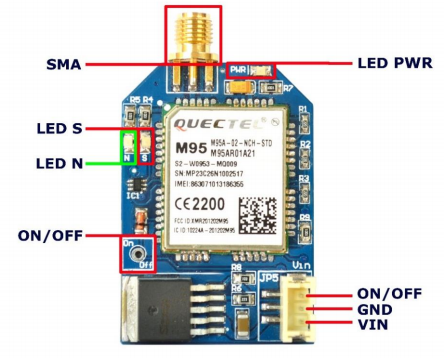
\includegraphics[scale=0.8]{figuras/com/gprs.png}
\caption{Modulo GPRSBee}
\label{gprs}
\end{figure}

Cabe destacar que para poder utilizar este m�dulo es necesario incluir una antena que se puede ver en la figura \ref{antena}

\begin{figure}[H]
\centering
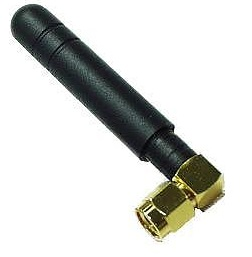
\includegraphics[scale=0.5]{figuras/com/antena.jpg}
\caption{Antena GPRSBee}
\label{antena}
\end{figure}

Al considerar este m�dulo se puede concluir que es incompatible con el dise�o del wearable ya que la antena es muy grande (aproximadamente $57.40[mm]$ ) lo que ser�a molesto en el dispositivo final. Otro punto en contra de este m�dulo es el alto costo y el consumo energ�a que lo hace incompatible con la autonom�a que se desea.

\subsection{Celular indirecta: Bluetooth BLE shield}
Para integrar Bluetooth en el dispositivo se considera un BLEBee el cual ofrece Bluetooth versi�n 4.1 y comunicaci�n UART mediante un puerto XBEE. \\
El shield Bluetooth posee un m�dulo RN4020\cite{RN4020} el cual ofrece una antena para la comunicaci�n en su misma placa lo que facilita el dise�o como se puede observar en la figura \ref{bt}.

\begin{figure}[H]
\centering
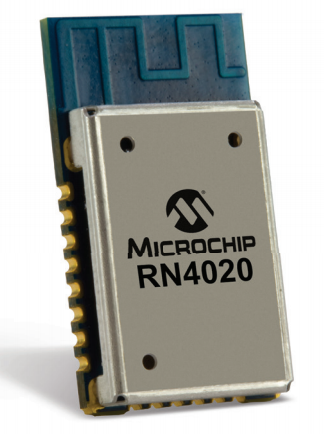
\includegraphics[scale=0.5]{figuras/com/rn4020.png}
\caption{Bluetooth RN4020}
\label{bt}
\end{figure}

Es importante destacar que para mejorar el dise�o, el fabricante recomienda dejar expuesta la antena y se destaca la comunicaci�n UART para las configuraciones futuras del sistema.

\newpage

\section{Conclusiones}
En esta secci�n, tomando en cuenta las opciones vistas en el mismo cap�tulo, se seleccionar�n las primeras componentes a utilizar para el prototipo funcional y para realizar la prueba de concepto con lo que se va a basar el proyecto.
\subsection{Plataforma de desarrollo}
Para la plataforma de desarrollo se va a escoger trabajar con Arduino ya que este posee distintas versiones con distintos costos, los cuales son menores que Raspberry o Beaglebone. Adem�s cabe destacar que el sistema que se quiere desarrollar es toma de datos y env�o de informaci�n por lo que no se va a requerir tanto procesamiento. Arduino cubre las necesidades en su versi�n UNO con un microcontrolador ATMega328p, en caso de necesitar uno de mayor capacidad se puede optar por un Arduino Mega.
\subsection{Electrocardiograma}
Para el sensor de electrocardiograma se utilizar� el monitor de actividad card�aca de DFRobot, esto debido a que es la �nica opci�n que se puede conseguir en el pa�s para no retrasar el desarrollo. Este sensor es de muy bajo costo (alrededor de 19.500 CLP en MCIElectronics).
El integrado ADS1298 es una buena opci�n como una mejora para una segunda iteraci�n del dise�o para mejorar la se�al que se puede obtener debido a que este posee mayor tolerancia al ruido. Se debe destacar esta �ltima opci�n debido a que se debe encargar directamente desde Texas Instruments y esto puede tomar mucho tiempo.
\subsection{Temperatura}
En primera instancia se va a utilizar el sensor Lilypad ya que este est� dise�ado espec�ficamente para wearables adem�s de que utiliza un hilo conductor para unir sus terminales con la alimentaci�n y la toma de datos. Este sensor tiene un valor aproximado de 3.790 CLP.\\
Dependiendo de los resultados obtenidos en la primeras pruebas se va a evaluar la segunda alternativa de utilizar el DS18B20 el cual tiene un valor aproximado de 5.900 CLP.
\subsection{IMU}
Al buscar las alternativas que existen en el pa�s, todas las opciones de desarrollo usan distintas placas de desarrollo pero utilizan el mismo sensor MPU-9250 por lo que se va a utilizar la placa de Sparkfun MPU-9250 luego de tener el prototipo funcional con los primeros sensores de electrocardiograma y temperatura. Esta placa de desarrollo tiene un valor aproximado de 12.500 CLP.
\subsection{Comunicaci�n}
Entre las alternativas mencionadas, se opta por utilizar en primera instancia el GPRS shield, el cual posee un costo aproximado de 43.980 CLP.
Cabe mencionar que en una segunda instancia se utilizar�a el chip RN4020, el cual posee un precio aproximado de 20.000 CLP.\\
Si bien el costo es menor, es relevante la complejidad que agrega la segunda opci�n (al agregar un actor como lo puede ser un tel�fono inteligente), es este criterio el que nos lleva a priorizar de esta forma la elecci�n en este punto.

\newpage
%---------------------------------------------------------------------------------------
\chapter{Selecci�n del microcontrolador}\label{chap5}
Se determin� utilizar la plataforma Arduino por su simplicidad en prototipado y programaci�n, adem�s de ser de f�cil acceso y una tecnolog�a escalable.
\section{ATMega328p}
Utilizando una placa Arduino Uno se comienza el prototipo del dispositivo que va a cumplir la funci�n de tomar los datos de los sensores an�logos. La versi�n de Arduino Uno utiliza un microcontrolador ATMega328 que posee 32[KB] de memoria de programa y una memoria RAM de 2[Mb]. Este consta de 1 puerto de comunicaci�n UART y posee 32 pines de los cuales 23 pines son programables para entrada/salida como se muestra en la figura \ref{328}

\begin{figure}[H]
\centering
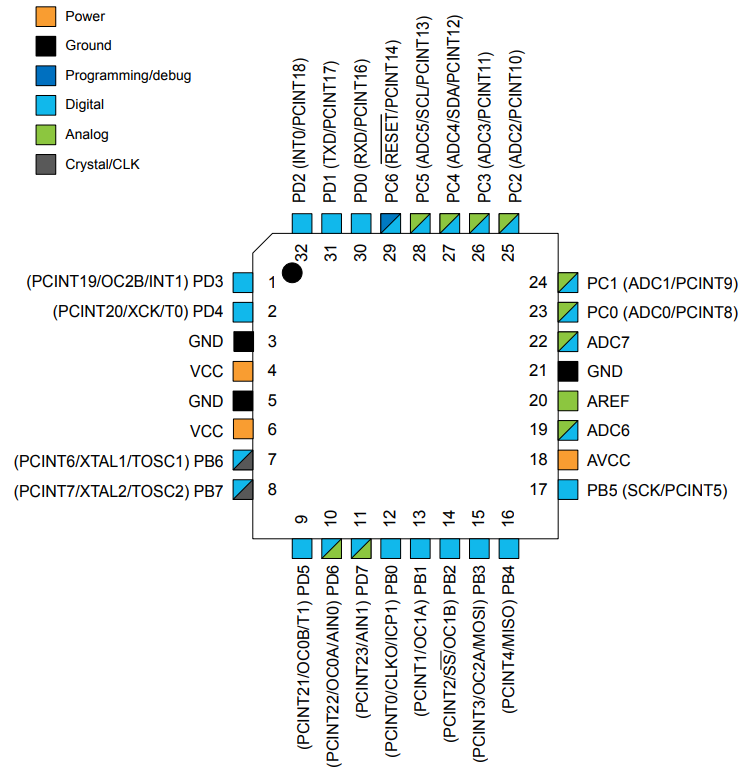
\includegraphics[scale=0.35]{figuras/mcu/328.png}
\caption{Microcontrolador ATMega328p}
\label{328}
\end{figure}

\section{ATMega2560}
Contrastando el modelo mostrado anteriormente, la placa Arduino Mega posee un microcontrolador ATMega2560 el cual incluye un aumento en todas sus capacidades. Comenzando con la capacidad de su memoria de programa, que asciende a 250[KB] y una memoria RAM de 8[KB]. Este microcontrolador posee 100 pines lo que incluye un aumento a 4 puertos de comunicaci�n UART, adem�s de aumento de entradas an�logas y digitales. 

\begin{figure}[H]
\centering
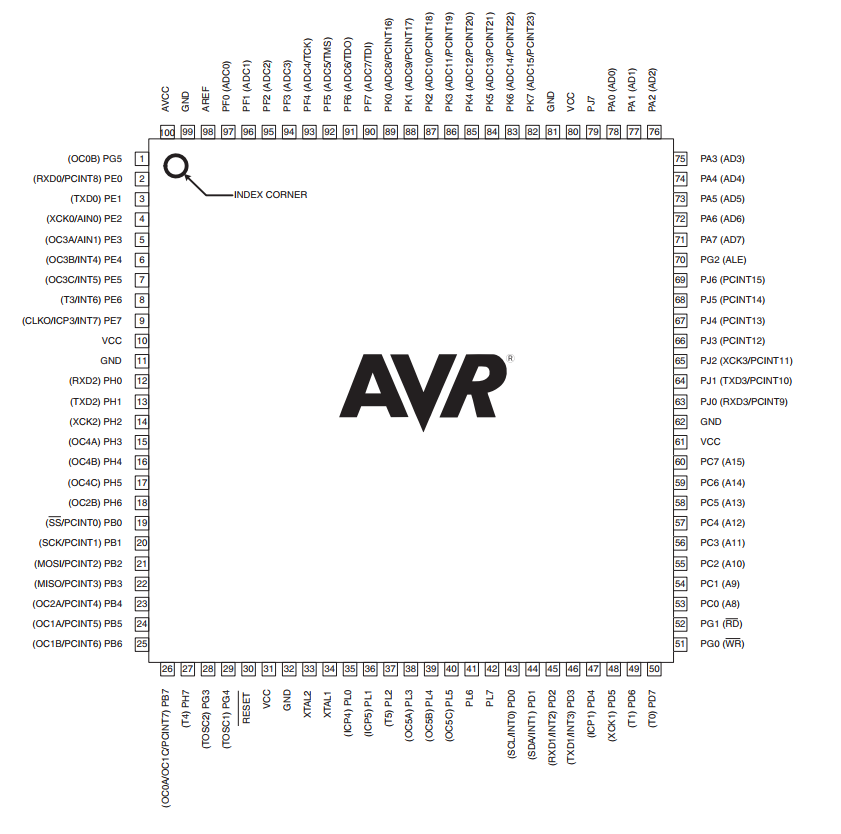
\includegraphics[scale=0.5]{figuras/mcu/2560.png}
\caption{Microcontrolador ATMega2560}
\label{mega}
\end{figure}

Como se puede observar en la figura \ref{mega}, hay un aumento considerable en las prestaciones que ofrece este microcontrolador con respecto al ATMega328p adem�s de su tama�o. \\

Se va a trabajar en el dise�o con este microcontrolador ya que posee 4 interfaces UART de las cuales una de estas siempre est� definida para ser utilizada por la programaci�n FTDl, esto se explicar� mas adelante.\\

Esto involucra utilizar un chip con mayores capacidades de las necesarias pero esto es debido a la limitante de los microcontroladores utilizados por Arduino como se puede observar en la figura \ref{compara}.

\begin{figure}[H]
\centering
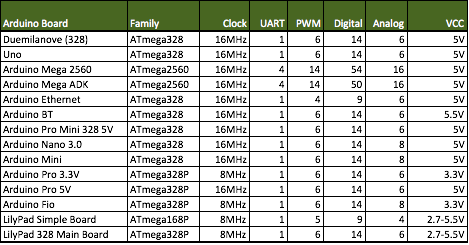
\includegraphics[scale=0.7]{figuras/mcu/compara.png}
\caption{Comparaci�n microcontroladores Arduino}
\label{compara}
\end{figure}

Idealmente para el dise�o del dispositivo, se utilizar� un microcontrolador con 2 puertos UART ya que uno de estos es necesario para la comunicaci�n con el computador y el otro es utilizado para el env�o de informaci�n mediante bluetooth, pero por necesidad de rapidez para el dise�o de prototipo y pruebas de sensores es necesario iterar con una placa ya fabricada para usos generales y disponibles en el mercado. Esto causar�a una disminuci�n significativa entre el precio del dise�o del producto final. 
\newpage
\section{ATMega644PA}
Considerando la variable de costos es importante destacar una tercera opci�n para el dise�o del dispositivo final. El microcontrolador ATMega644PA posee un menor conteo de pines ya que consta de 44 lo cual disminuye costos y tama�o a la hora del dise�o. Con una memoria Flash de 64[KB] y memoria RAM de 4[KB]. Este provee 2 UART para la comunicaci�n y los pines suficientes para sensores como se muestra en la figura \ref{644}.

\begin{figure}[H]
\centering
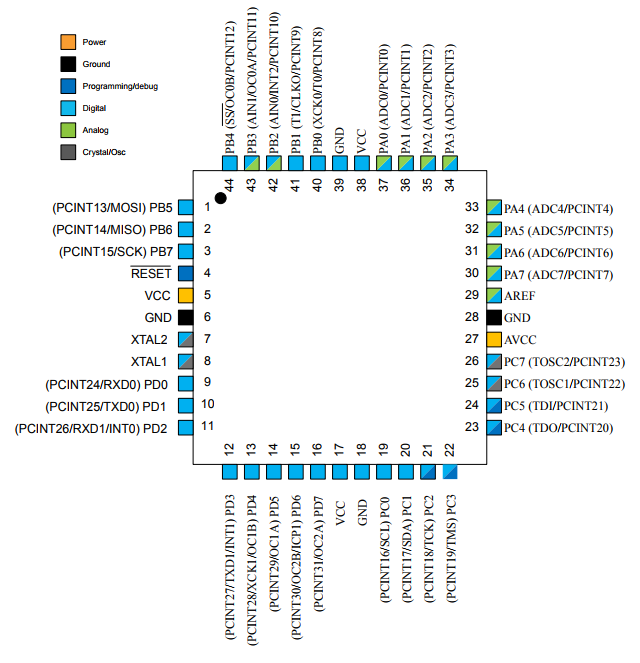
\includegraphics[scale=0.7]{figuras/mcu/644.png}
\caption{Microcontrolador ATMega644PA}
\label{644}
\end{figure}

Se puede observar en la imagen la disponibilidad de los puertos UART donde el Pin 9 y Pin 10 corresponden a UART0 considerado para la programaci�n USB. Pin 11 y Pin 12 corresponden a UART1 que ser� utilizado para la comunicaci�n con el dispositivo bluetooth.\\
En primera instancia se va a dise�ar el dispositivo con el microcontrolador ATMega2560, debido a que existen modelos Arduino con esta misma componente y cumple los requisitos funcionales de poseer mas de 1 puerto UART. No es la opci�n ideal ya que posee mas prestaciones de las que se necesitan pero permite que se pueda prototipar inmediatamente  utilizando un Arduino equivalente, lo cual no se puede hacer con la versi�n ATMega644PA.

\section{Conclusiones}
Finalmente considerando las 3 opciones elegidas, se puede establecer una decisi�n final con respecto a cual microcontrolador utilizar.


\begin{table}[H]
\centering
\begin{tabular}{| c | c | c |}
\hline
\multicolumn{1}{|c|}{\textbf{Microcontrolador}}&
\multicolumn{1}{c|}{\textbf{Pines}}&
\multicolumn{1}{|c|}{\textbf{Precio (USD)}}\\ \hline
ATMega328p  & 32  & \$2.18  \\ \hline
ATMega2560  & 100 & \$12.44 \\ \hline
ATMega644PA & 44  & \$5.24  \\ \hline
\end{tabular}
\caption{Comparaci�n microcontroladores}
\label{tablacompara}
\end{table}

Como se puede observar en la Tabla 1 se tomaron en cuenta los aspectos de tama�o y costos. ATMega328p se considera porque a pesar de que posee un solo puerto UART es posible utilizar otros pines para configurar comunicaci�n serial por software (en comparaci�n con la comunicaci�n por hardware es mucho m�s lenta) lo cual ser� muy �til a la hora de hacer pruebas en toma de datos y env�o de la informaci�n. En cuanto a precio y tama�o es una alternativa ideal ya que minimiza ambos aspectos. \\
La segunda opci�n siendo la que ofrece m�s opciones para sensores y memoria programable es excesivo para lo que se necesita desarrollar, pero se acerca m�s a los requerimientos necesarios que carece el microcontrolador ATMega328p. Esta opci�n tiene un el precio m�s elevado de las 3 opciones y por una diferencia considerable, es por esto que se utilizar� para la primera versi�n del dise�o final enfocado a tener un m�nimo producto viable que funcione de la misma manera que el prototipo.\\
Finalmente la tercera opci�n siendo la m�s viable ya que posee un tama�o mucho menor al ATMega2560 y un precio menor a la mitad que este, ofrece todas las capacidades necesarias pero como se muestra en la figura \ref{compara}, no hay en el mercado una placa Arduino con este microcontrolador ni tampoco otra opci�n que cumpla con el requisito de utilizar 2 UART es por esto que como segunda iteraci�n del producto final se debe buscar un bootloader compatible con el entorno de desarrollo Arduino para el ATMega644PA o trabajar en otra plataforma compatible con ese microcontrolador.




\newpage
% ---------------------------------------------------------------------------------------
\chapter{Firmware y programaci�n del microcontrolador}\label{chap6}
Los microcontroladores Arduino son usados en el dise�o de sistemas embebidos para distintas funciones. El microcontrolador es un peque�o chip que posee pines con funciones de lectura y escritura, memoria, entradas y salidas. Mientras los microcontroladores han sido usados por d�cadas, los microcontroladores Arduino son utilizados actualmente ya que permiten ejecutar funciones electr�nicas sin necesidad de conocer hardware y software integrado en estos. 
\section{Bootloader}
Dentro de las m�ltiples definiciones que existen con respecto al bootloader, lo m�s com�n es considerarlo como un software o firmware que reside parcialmente en la memoria no vol�til del microcontrolador, como la ROM o memoria Flash. \\
En la pr�ctica el bootloader empieza a funcionar justo despu�s de prender el microcontrolador o despu�s de reiniciarlo. \\
Este bootloader va a ser el que va a permitir la programaci�n del circuito con el entorno de desarrollo Arduino (Arduino IDE) manejando de mejor manera la toma de datos por medio de las entradas an�logas, el procesamiento y la comunicaci�n.

\newpage
\section{ISP - In-System Programming}
Tambi�n conocido como programaci�n serial en circuito\cite{isp} (ICSP), es la habilidad de algunos dispositivos l�gicos programables, microcontroladores y otros circuitos electr�nicos de ser programados mientras est�n instalados en un sistema completo, no es necesario programar el chip antes de instalarlo en el sistema. Esto permite armar un circuito con todo lo que se desea y programarlo en el circuito impreso.\\
T�picamente los chips que soportan programaci�n ISP tienen circuiter�a interna que genera el voltaje necesario y permite comunicarse con el programador a trav�s de protocolo serial.
La mayor�a de los dispositivos l�gicos programables usan una variante del protocolo JTAG para ISP para facilitar la integraci�n con procedimientos automatizados de pruebas.\\
JTAG (Joint Test Action Group) es una interfaz dise�ada originalmente para circuitos impresos y es muy �til tambi�n como mecanismo para depuraci�n de aplicaciones embebidas, puesto que provee una puerta trasera para acceder al sistema. El m�dulo de depuraci�n permite al programador corregir errores de c�digo y de l�gica de sus sistemas.\\

\begin{figure}[H]
\centering
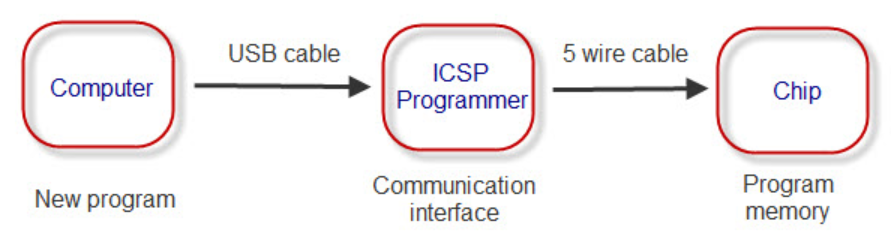
\includegraphics[scale=0.5]{figura/firmware/isp.png}
\caption{Configuraci�n ISP para programar un microcontrolador}
\label{isp}
\end{figure}

Se observa en la Figura \ref{isp} un simple diagrama de flujo donde es importante destacar que para poder programar un chip es necesaria una conexi�n de 5 cables entre un intermediario que viene a ser el programador ICSP (o ISP) y el chip (Microcontrolador).

\newpage
\section{Programaci�n de un microcontrolador}
Para que el entorno de desarrollo Arduino reconozca el microcontrolador como una placa Arduino, es necesario grabar el bootloader en este. Se escribe el bootloader en la memoria del microcontrolador mediante la comunicaci�n ISP que se muestra en la figura \ref{pin}.

\begin{figure}[H]
\centering
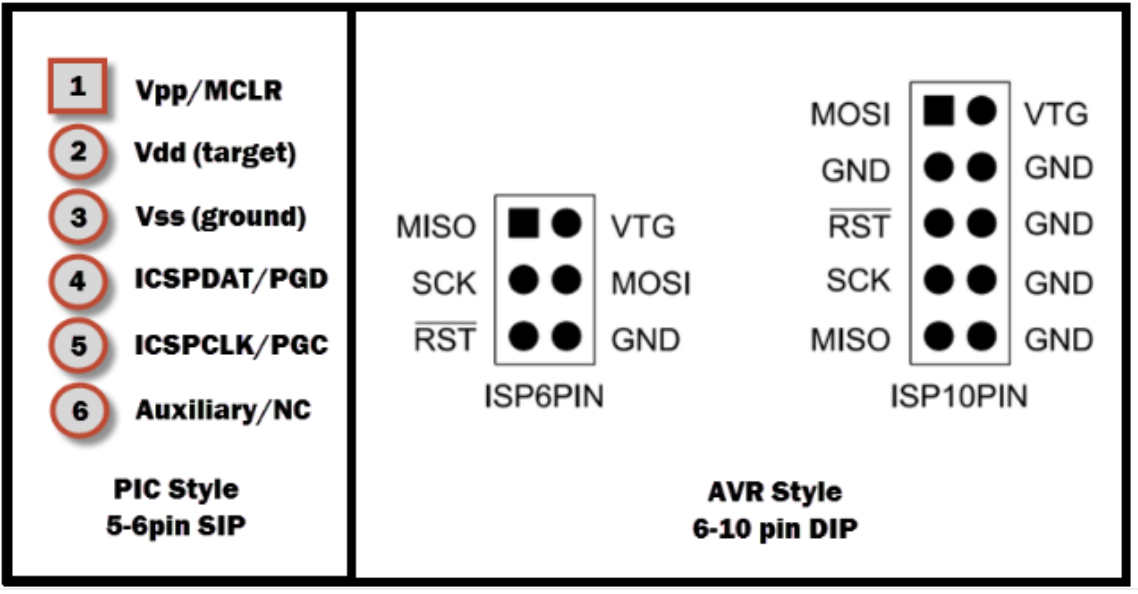
\includegraphics[scale=0.5]{figura/firmware/pin.png}
\caption{Conector t�pico para programaci�n ISP}
\label{pin}
\end{figure}

La figura \ref{pin} muestra el conector ISP que se va a encargar de cargar el bootloader en el microcontrolador.  En este caso se est� utilizando la tecnolog�a AVR (microcontrolador ATMega) la cual es usada por las placas Arduino y es por esto que se usar� la configuraci�n de 6 pines. 

\begin{figure}[H]
\centering
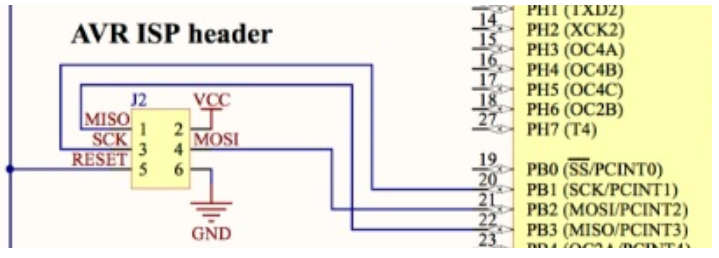
\includegraphics[scale=0.6]{figura/firmware/eagleisp.png}
\caption{Esquem�tico b�sico MCU con ISP}
\label{eagle11}
\end{figure}

En la figura \ref{eagle11} se muestra una parte del esquem�tico con la configuraci�n b�sica en el microcontrolador AVR.
Se puede observar el diagrama de conexi�n del bus con el microcontrolador. Esto se puede observar con mayor detalle en la tabla \ref{tablaisp}\\

\subsection{Programador ISP}
 Existen varias alternativas que cumplen esta funci�n y dependen tanto del microcontrolador como del fabricante. Un microcontrolador AVR (Atmel) requiere de un programador STK500 con una interfaz serial RS232 (Existen otros programadores pero cumplen la misma funci�n, el STK500 es el m�s utilizado y posee mayor compatibilidad). Para programar un microcontrolador de Microchip se requiere de un PICkit.\\ 
Una segunda alternativa es utilizar un Arduino ya programada que cumpla la funci�n del programador. Estas vienen con un puerto ISP el cual permite cargar el bootloader en el microcontrolador. Respetando la misma conexi�n que se muestra en la figura \ref{eagle11}.\\

\begin{table}[H]
\centering
\begin{tabular}{| c | c | c |}
\hline
\multicolumn{1}{|c|}{\textbf{AVR ISP}}&
\multicolumn{1}{c|}{\textbf{Arduino UNO}}&
\multicolumn{1}{|c|}{\textbf{ATMega2560}}\\ \hline
1 & MISO  & Pin 22 \\ \hline
2 & VCC   & VCC    \\ \hline
3 & SCK   & PIN 20 \\ \hline
4 & MOSI  & Pin 21 \\ \hline
5 & RESET & Pin 30 \\ \hline
6 & GND   & GND    \\ \hline
\end{tabular}
\caption{Programaci�n ISP utilizando Arduino UNO}
\label{tablaisp}
\end{table}

\section{Programaci�n USB}
La compa��a escocesa Future Technology Devices International (FTDI) est� especializada en la tecnolog�a USB (Universal Serial Bus). Esta ofrece chips encargados de transformar una conexi�n USB a un puerto UART y esto ser� fundamental a la hora de programar el dise�o final con el programa en el entorno Arduino.
\newpage
\subsection{FT232RL}
El Chip FT232RL\cite{ft232} ofrece una conversi�n USB-UART y cuenta con 28 pines como se muestra en la figura \ref{ft232ft}.

\begin{figure}[H]
\centering
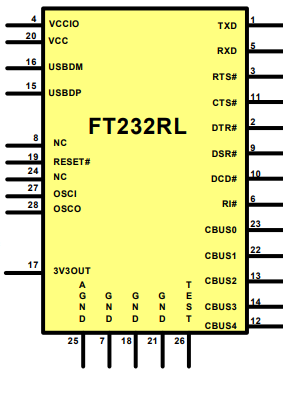
\includegraphics[scale=0.6]{figura/firmware/ft232.png}
\caption{Chip FT232RL}
\label{ft232ft}
\end{figure}

En la tabla \ref{ft232} se muestra la descripci�n de los pines m�s importantes para la conexi�n del FTDI con el microcontrolador y al mismo tiempo con el USB para permitir la programaci�n del chip. 

\begin{table}[H]
\centering
\begin{tabular}{| c | c | c | c |}
\hline
\multicolumn{1}{|c|}{\textbf{N� Pin}}&
\multicolumn{1}{c|}{\textbf{Nombre}}&
\multicolumn{1}{|c|}{\textbf{Descripci�n}}\\ \hline
1  & TXD    & Transmisor de datos UART \\ \hline
5  & RXD    & Receptor de datos UART    \\ \hline
4  & VCCIO  & 1.8[V] a 5.25[V] alimentaci�n a la interfaz UART y a los pines CBUS \\ \hline
15 & USBDP  & Conexi�n Data+ USB \\ \hline
16 & USBDM  & Conexi�n Data- USB \\ \hline
17 & 3V3OUT & Regulador de voltaje interno.    \\ \hline
22 & CBUS1  & Indicador de funcionamiento RXD   \\ \hline
23 & CBUS2  & Indicador de funcionamiento TXD    \\ \hline
\end{tabular}
\caption{Descripci�n de pines chip FT232RL}
\label{ft232}
\end{table}

Este chip ser� encargado de conectar la interfaz UART (TX y RX) con el microcontrolador adem�s de permitir la comunicaci�n con la conexi�n USB (USBDP y USBDM).\\
Al trabajar con una conexi�n USB se tiene conexi�n con VCC y GND desde el computador que est� programando y este provee una alimentaci�n de 5[V]. Este voltaje es com�nmente utilizado en los microcontroladores pero adem�s provee un regulador de voltaje interno de 3.3[V] el cual est� disponible si se est� trabajando con un sistema con menor voltaje.
En caso de utilizar voltaje 3.3[V] para todo el sistema, es necesario conectar el pin 3V3OUT a VCCIO utilizando un condensador de 100[nF] como se indica en el manual. De esta forma la alimentaci�n del microcontrolador es la misma que la alimentaci�n FTDI para la programaci�n UART y no se da�an las componentes.

\begin{figure}[H]
\centering
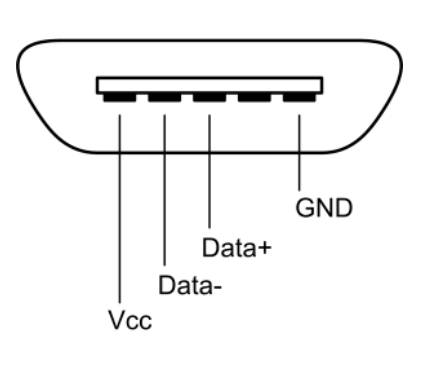
\includegraphics[scale=0.6]{figura/firmware/usb.png}
\caption{Conector USB 2.0 Micro B}
\label{usb}
\end{figure}

Se muestra en la figura \ref{usb} las 4 conexiones que posee un conector USB, las cuales son la alimentaci�n VCC, GND y la conexi�n de datos Data+ (USBDP en FT232) y Data- (USBDM en FT232). 

\newpage
\section{Programa en Arduino}

Para la programaci�n del Arduino se trabaj� en conjunto con la parte telem�tica del grupo. Se realiz� la programaci�n de la toma de datos de los sensores. Adem�s de un algoritmo antirebote para pedir toma de muestras en el prototipo que luego fue sustituido por una orden emitida por la aplicaci�n. Este c�digo se puede observar en el anexo. En esta parte se puede observar la divisi�n de las tareas en el grupo debido a que esta memoria est� enfocada al area de dise�o de hardware mayoritariamente por lo que este c�digo no se explicar� en mayor profundidad.

\newpage
% ---------------------------------------------------------------------------------------
\chapter{Dise�o Electrocardiograma}\label{chap3}
El ECG (Electrocardiograma) detecta se�ales del cuerpo gracias a electrodos que se colocan en la superficie del cuerpo, usualmente acompa�ados de un gel conductor que elimina interferencia de los m�sculos, fuente de alimentaci�n,  ruido externo, etc. Para que se obtenga una se�al de ECG sin distorsiones excesivas, es necesario dise�ar filtros que eliminen interferencias antes de analizar la informaci�n. \\

\section{DFRobot Heart Rate Monitor}\label{reqfuncional1asc}
El monitor de actividad card�aca de la empresa DFRobot consiste en una placa que consta de un chip AD8232 en su PCB, el cual provee una clara se�al de los intervalos PR y QT (Ver Figura \ref{onda})  de un electrocardiograma. Este entrega un valor an�logo que puede ser le�do por Arduino y con un conversor an�logo-digital interpretarse en forma de gr�fico.\\

\begin{figure}[H]
\centering
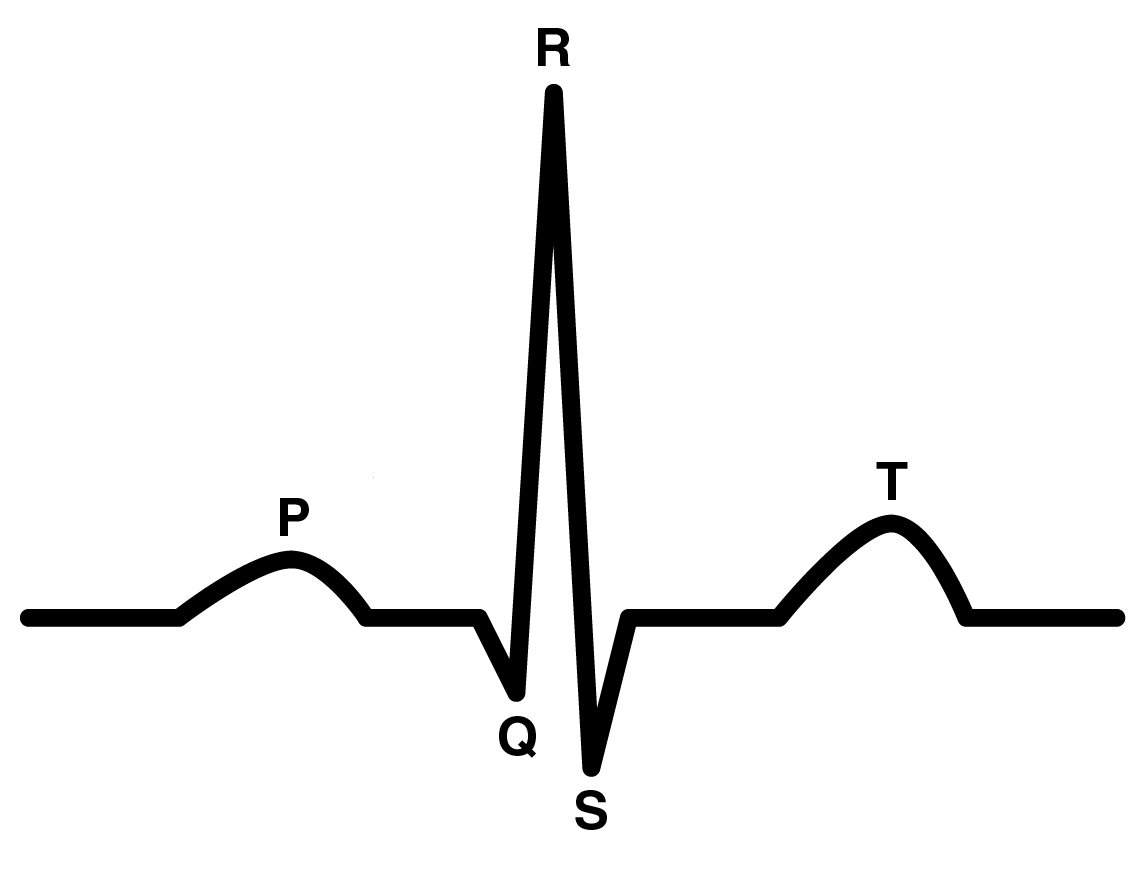
\includegraphics[scale=0.2]{figuras/ecg/senal.png}
\caption{Forma de onda te�rica ECG}
\label{onda}
\end{figure}

Se escogi� esta placa de desarrollo por disponibilidad de hardware, ya que es la �nica opci�n disponible de bajo costo, y que no necesita comprarse fuera del pa�s. Por lo que se tom� la decisi�n de estudiar su funcionamiento, replicarlo para el dise�o del dispositivo final y evaluar posibles mejoras. \\

\section{Biopac MP150 ECG100C}
Se tuvo la oportunidad de usar el ECG de la empresa Biopac ECG100C, el cual es de mucho mayor costo y tama�o utilizado generalmente para investigaci�n. La idea era ver la forma de onda y comparar las frecuencias de corte utilizadas. La figura \ref{biopac} muestra el aparato encargado de tomar las se�ales de los electrodos y la figura \ref{frecuencias} muestra un acercamiento con las posibles frecuencias de corte configurables para los filtros.\\

\begin{figure}[H]
\centering
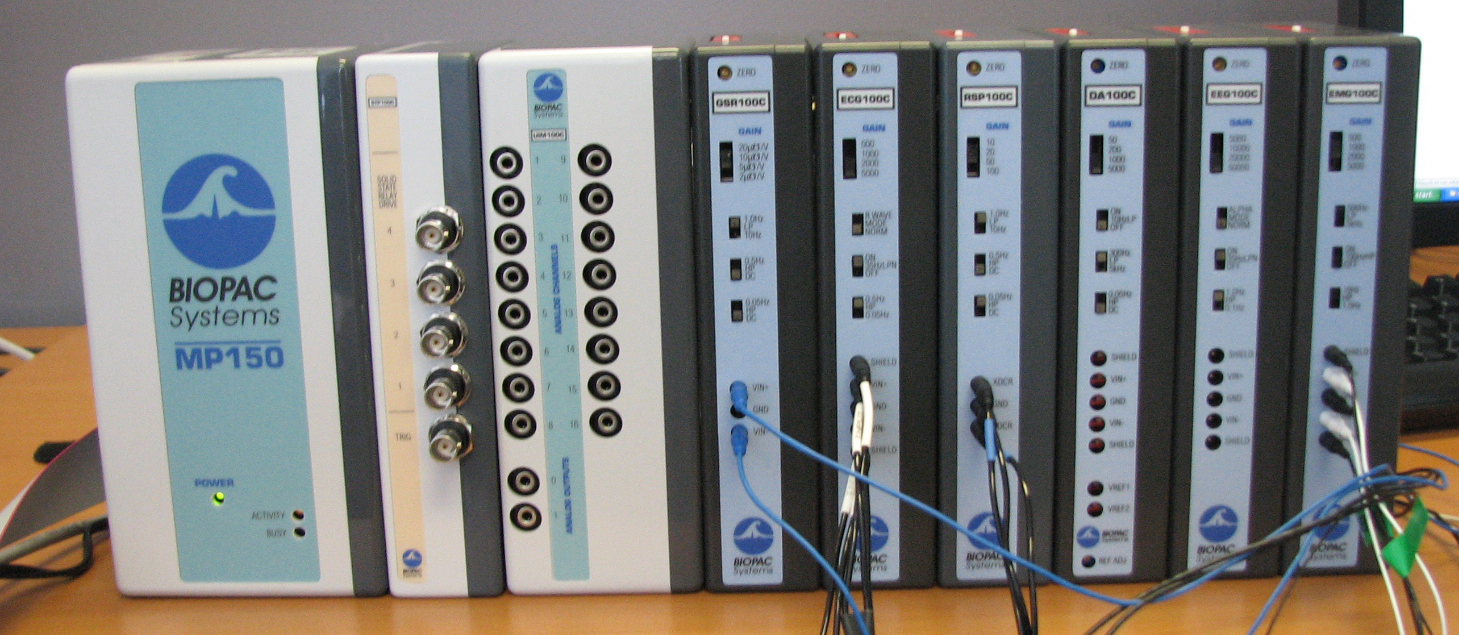
\includegraphics[scale=0.7]{figuras/ecg/biopac.jpg}
\caption{Biopac MP150}
\label{biopac}
\end{figure}

\begin{figure}[H]
\centering
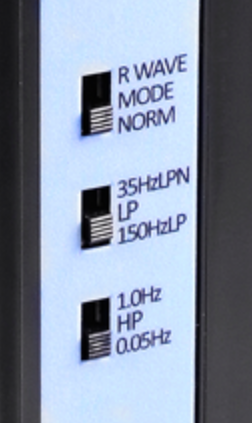
\includegraphics[scale=0.7]{figuras/ecg/biopacecg.png}
\caption{Frecuencias de corte disponibles en Biopac ECG100C}
\label{frecuencias}
\end{figure}

Cabe destacar el alto precio de este equipo que es de 45.000 USD y grandes dimensiones ya que est� dise�ado para investigaci�n lo cual servir� para saber donde tiene que apuntar la forma de onda de un ECG de grado m�dico.\\

\newpage
\section{AD8232}
El chip AD8232 es un integrado que permite medir las se�ales de los electrodos del ECG mediante amplificadores operacionales como se muestra en la figura \ref{ad8232}.

\begin{figure}[H]
\centering
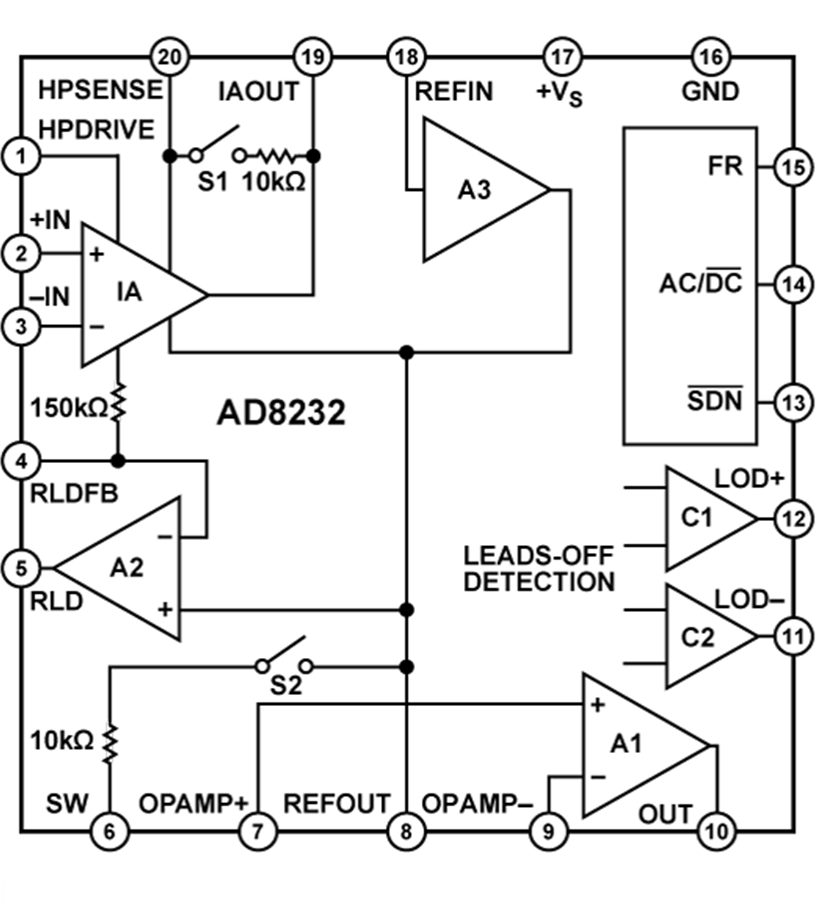
\includegraphics[scale=0.4]{figuras/ecg/ad8232.png}
\caption{Diagrama de bloques funcional}
\label{ad8232}
\end{figure}

Esta figura representa el funcionamiento del integrado y el proceso que realiza en su interior desde el punto de vista de los pines. 
A partir de este diagrama y la herramienta que provee el fabricante para el dise�o de filtros, se puede llegar a una configuraci�n del integrado con componentes pasivas para el dise�o del circuito impreso como se muestra en la figura \ref{ecgdesign}.\\

\begin{figure}[H]
\centering
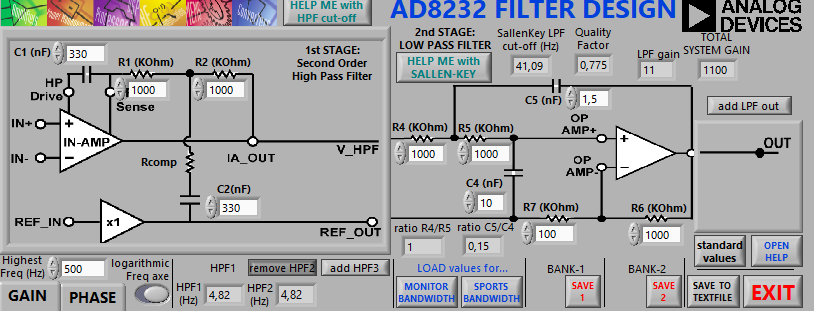
\includegraphics[scale=0.6]{figuras/ecg/ecgdesign.png}
\caption{Herramienta para dise�o de filtros}
\label{ecgdesign}
\end{figure}

Como se puede observar en la figura \ref{ecgdesign}, en el lado izquierdo se dise�a un filtro pasa alto de segundo orden cuya frecuencia de corte es de 4.82[Hz]. A la derecha se muestra un filtro pasabajo sallen-key con frecuencia de corte 41.09[Hz] donde finalmente se tiene una salida hacia el Arduino. 
Estos valores se obtuvieron al ver el circuito de la PCB de DFRobot (Figura \ref{esquematico11}) y utilizando la herramienta de dise�o de filtros. En caso de que se quisieran cambiar las frecuencias de corte se podr�a hacer un nuevo dise�o utilizando el mismo programa pero cambiando y apuntando a frecuencias de corte entre 1-35[Hz] dadas por el dispositivo Biopac.

\begin{figure}[H]
\centering
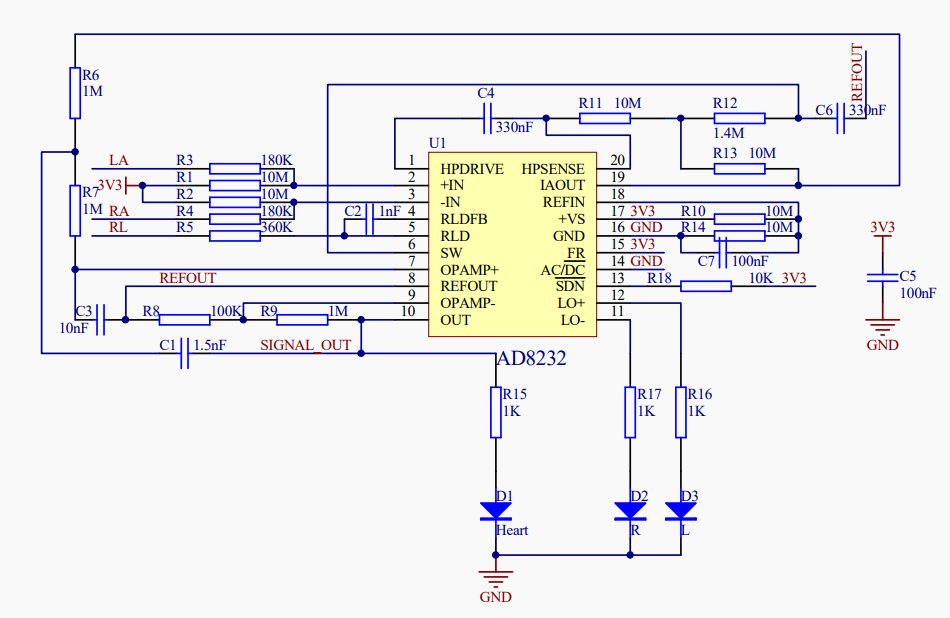
\includegraphics[scale=0.45]{figuras/ecg/esquematico.png}
\caption{Esquem�tico ECG DFRobot}
\label{esquematico11}
\end{figure}

\newpage
\section{Comparaci�n entre Biopac y DFRobot}
Finalmente se pudo contrastar ambas se�ales, se puede observar en la figura \ref{graficos} la se�al de ECG del Biopac y DFRobot colocando los electrodos muy cerca para obtener las se�ales lo m�s parecidas posibles y poder compararlas. 

\begin{figure}[H]
\centering
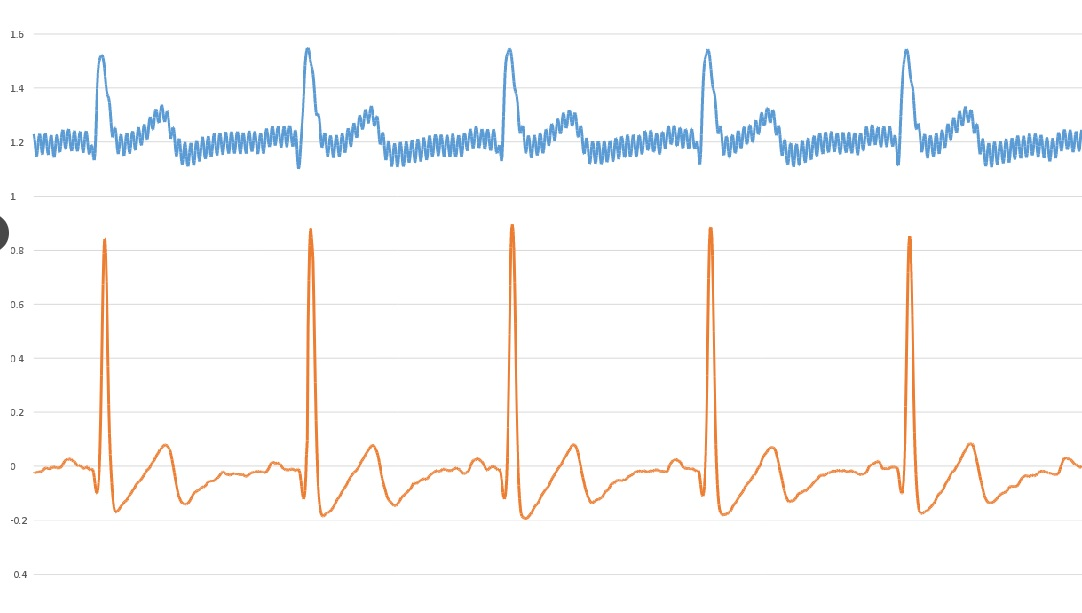
\includegraphics[scale=0.45]{figuras/ecg/biovsdf.jpg}
\caption{Gr�fico Biopac ECG100C vs ECG DFRobot}
\label{graficos}
\end{figure}

En el gr�fico superior se puede observar la forma de onda del ECG AD8232 en la cual se puede observar notoriamente un ruido de la fuente. En el gr�fico inferior se muestra la se�al del ECG100C de Biopac, la cual es una se�al muy definida a lo cual deber�a apuntar el dise�o del ECG.
Se puede concluir de estas im�genes que la forma de onda de ambas se�ales son parecidas, considerando que el Biopac est� dise�ado para mostrar la onda completa, en cambio el AD8232 se encarga de mostrar la onda PR y QT. 
Finalmente se considera que la forma de onda que se tiene sirve para hacer mediciones eliminando el ruido de la fuente ya que es representativa por los peaks que presenta. 

\section{Eliminando ruido de la fuente}
Observando la se�al que se tiene actualmente en el dispositivo mediante bluetooth en la aplicaci�n m�vil se obtiene una se�al como se observa en la figura \ref{ecgfeo}.

\begin{figure}[H]
\centering
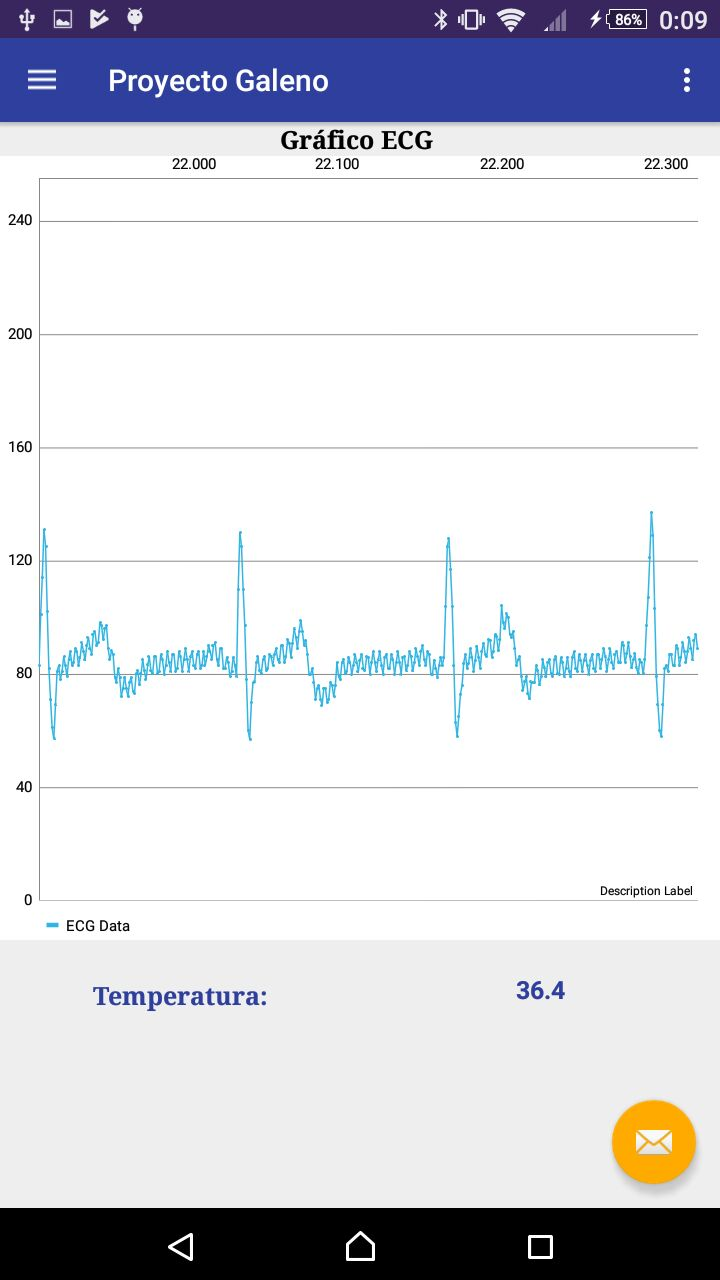
\includegraphics[scale=0.3]{figuras/ecg/ecgappmalo.jpg}
\caption{ECG en aplicaci�n m�vil sin filtro de salida}
\label{ecgfeo}
\end{figure}

Se puede notar en esta imagen que la forma de onda se mantiene al enviarla por bluetooth a la aplicaci�n pero sigue con mucho ruido. Utilizando la herramienta de dise�o de filtros para el AD8232 existe una opci�n para filtrar la salida de la se�al final, para esto se considera utilizar un filtro pasabajo para eliminar el ruido como se muestra en la figura \ref{filtroout}.

\begin{figure}[H]
\centering
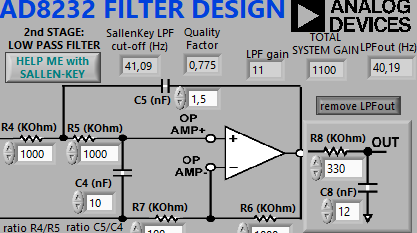
\includegraphics[scale=0.75]{figuras/ecg/filtroout.png}
\caption{Filtgro de salida R8 y C8}
\label{filtroout}
\end{figure}

Se dise�� con frecuencia de corte de $40.19[Hz]$ como se muestra en la figura \ref{filtroout} dando valores $R8 = 330[k\Omega]$ y $C8 = 12[nF]$ para no perder informaci�n de la se�al y con esto limpiar solamente la se�al como se muestra en el resultado de la figura \ref{ecgbonito}

\begin{figure}[H]
\centering
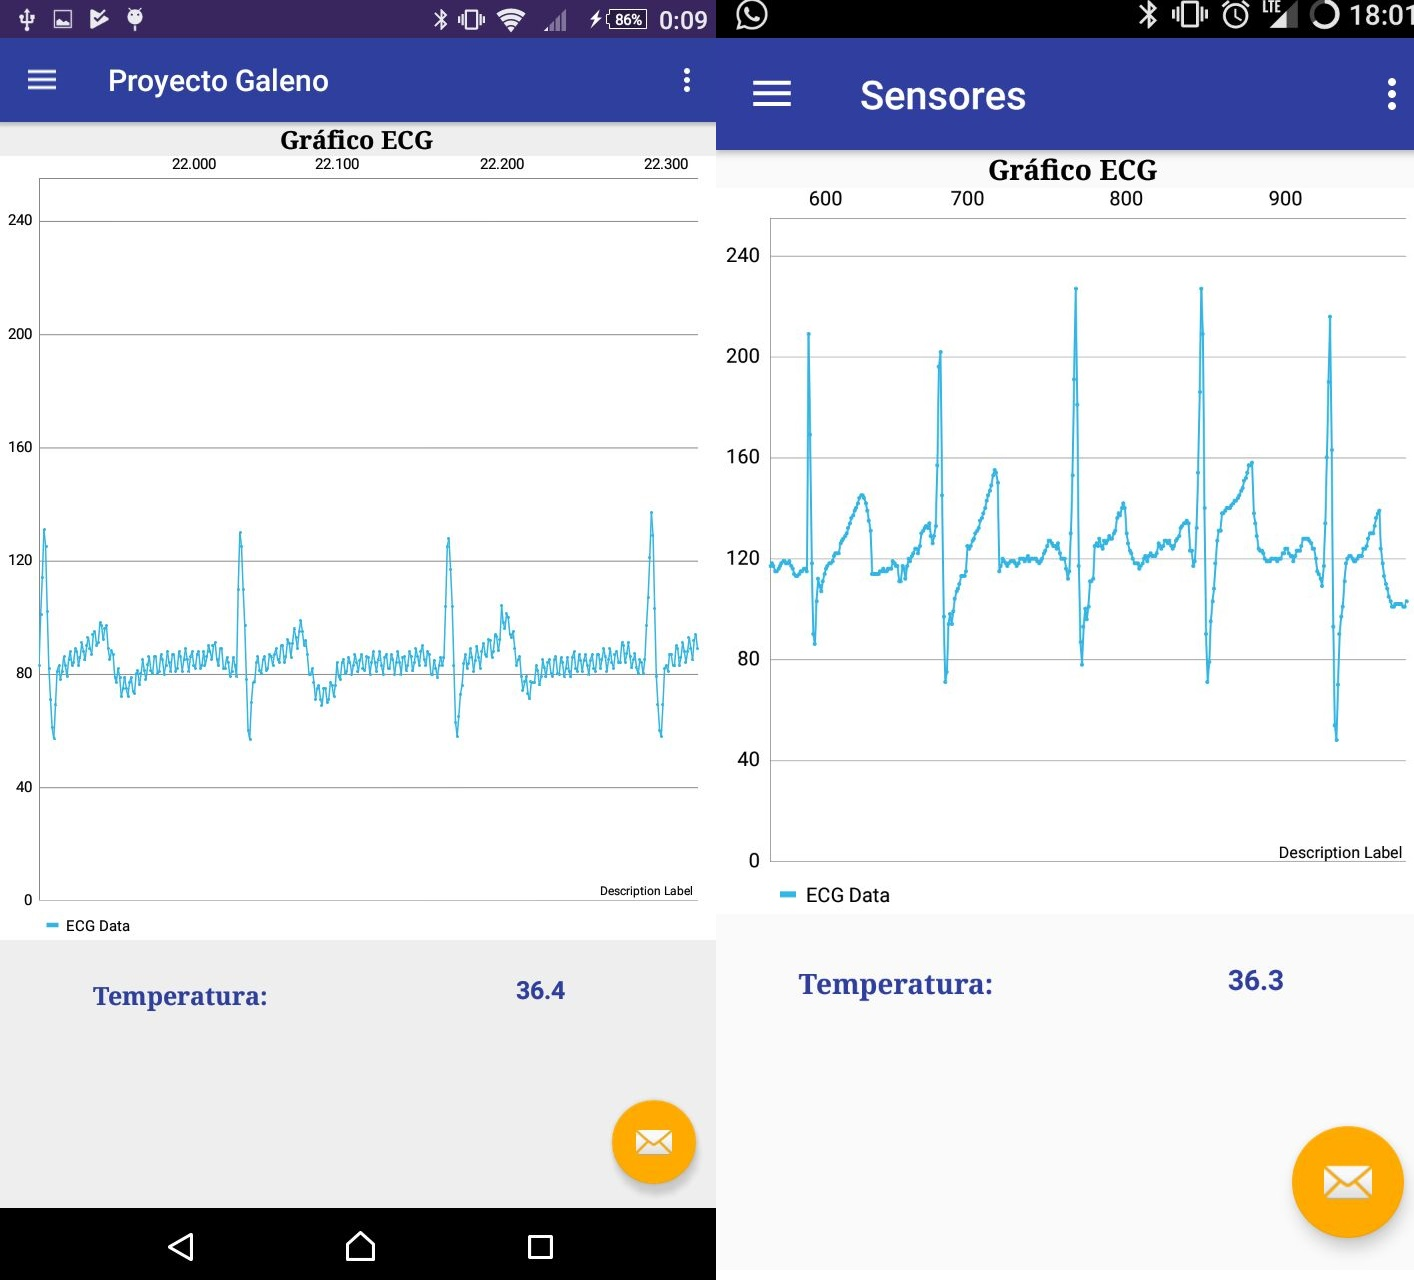
\includegraphics[scale=0.25]{figuras/ecg/ecgappbueno.jpg}
\caption{Comparaci�n ECG en aplicaci�n m�vil con filtros de salida}
\label{ecgbonito}
\end{figure}

Se nota un gran cambio en la forma de la se�al, donde se notan de mejor manera, sin ruido de la fuente y sin perder la forma de onda. Esta ser� la configuraci�n que se utilizar� para el dise�o final del dispositivo.



\newpage
% ---------------------------------------------------------------------------------------
\chapter{Dise�o bluetooth}\label{chap2}
En esta secci�n se abordar� el hardware utilizado para prototipado y dise�o de bluetooth bajo consumo (BLE - bluetooth low energy). 

\section{BLEBee}
Para el prototipado se utilizar� un m�dulo bluetooth BLEBee que ofrece una conexi�n simple a placas Arduino que posean este puerto. 
BLEBee utiliza un m�dulo de bluetooth RN4020 el cual ofrece bluetooth versi�n 4.1.\\
Mediante interfaz UART, este modulo puede ser configurado para actuar como m�dulo central o perif�rico cuando establezca una conexi�n.\\
Para conocer mas el funcionamiento de este m�dulo primero hay que conocer mejor la conexi�n XBee.

\begin{figure}[H]
\centering
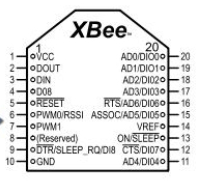
\includegraphics[scale=1]{figuras/bluetooth/xbee.png}
\caption{Forma y Pines de puerto XBee}
\label{xbee}
\end{figure}

Como se puede observar en la figura \ref{xbee} el puerto XBee ofrece una conexi�n de 20 pines con usos generales que se utilizan por distintos dispositivos, en este caso bluetooth.\\
En el caso de BLEBee la distribuci�n de los pines se puede observar en la figura \ref{blebee}

\begin{figure}[H]
\centering
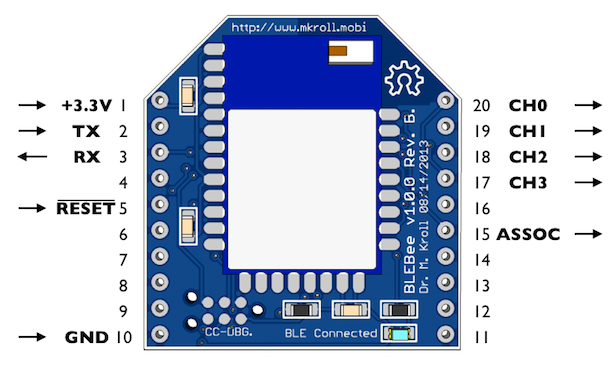
\includegraphics[scale=0.5]{figuras/bluetooth/blebee.png}
\caption{Distribuci�n de pines BLEBee}
\label{blebee}
\end{figure}

Comparando la figura \ref{xbee} con la figura \ref{blebee} se puede observar los pines mas relevantes a la hora de dise�ar un m�dulo bluetooth en el dispositivo, siendo los pines mas importantes, y contrastando con el datasheet, los que se muestran en la tabla \ref{pines}

\begin{table}[H]
\centering
\begin{tabular}{| c | c | c |}
\hline
\multicolumn{1}{|c|}{\textbf{N� Pin}}&
\multicolumn{1}{c|}{\textbf{Nombre}}&
\multicolumn{1}{|c|}{\textbf{Descripci�n}}\\ \hline
5  & UART TX & Transmisor UART\\ \hline
6  & UART RX & Receptor UART\\ \hline
7  & WAKE\_ SW & Despertador de modo deep sleep\\ \hline
10 & Led Conexi�n  & Led indicador de conexi�n\\ \hline
12 & Led Actividad & Led indicador de actividad\\ \hline
\end{tabular}
\caption{Pines relevantes m�dulo RN4020}
\label{pines}
\end{table}

\newpage
\section{Comunicaci�n UART}

La comunicaci�n UART (Universal Asynchronous Receiver-Transmitter) es un formato de comunicaci�n serial donde el formato y la velocidad de transmisi�n son configurables. Un UART puede ser un circuito integrado independiente pero en la actualidad vienen incluidos en los microcontroladores.\\
Para entender mejor como funciona la comunicaci�n serial mediante UART hay que observar la figura \ref{UART}

\begin{figure}[H]
\centering
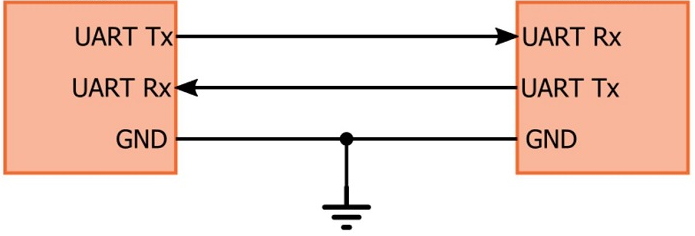
\includegraphics[scale=0.8]{figuras/bluetooth/uart.png}
\caption{Configuraci�n para comunicaci�n UART}
\label{UART}
\end{figure}

La comunicaci�n UART cuenta de 2 pines TX (transmisor) y RX (receptor) el cual se conecta al Receptor y transmisor del microcontrolador respectivamente.

\section{Dise�o del m�dulo bluetooth}
Finalmente contrastando lo visto anteriormente y con referente a la tabla \ref{pines} se puede dise�ar el esquem�tico del integrado.\\
Pin 5 y 6 corresponden a la comunicaci�n UART como se explica en la figura \ref{UART}. Es necesario conectar los pines 10 y 12 con diodos led ya que son pines indicadores, el pin 10 indica el estado de la conexi�n con un led verde y tambi�n se recomienda conectar un led azul al pin 12 para ver el estado de actividad (ej. Si se est� enviando informaci�n o est� dormido).\\
El pin 7 cumple la funci�n de despertar el m�dulo bluetooth cuando se encuentre dormido emitiendo desde el microcontrolador una se�al de $3.3[V]$.\\
\begin{figure}[H]
\centering
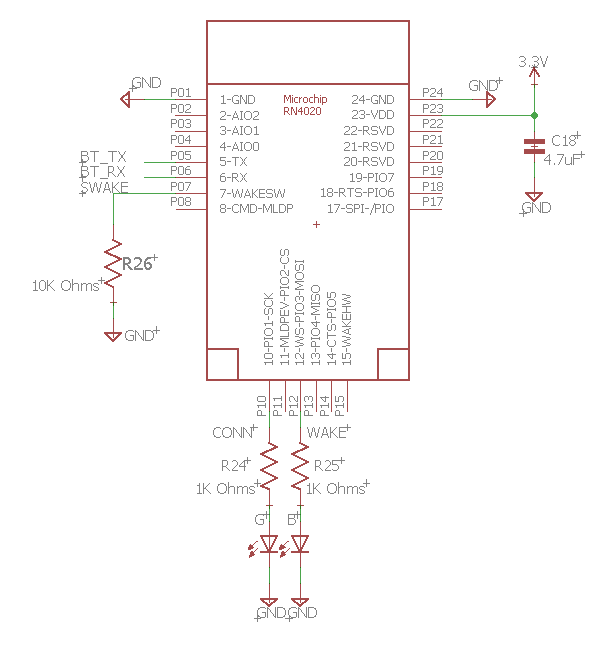
\includegraphics[scale=0.8]{figuras/bluetooth/eagle.png}
\caption{Esquem�tico bluetooth dise�ado en EagleCAD}
\label{eagle}
\end{figure}

Como se puede observar en la figura \ref{eagle} se conecta el m�dulo bluetooth con los pines descritos. Se utiliza un condensador en la alimentaci�n de m�dulo para regular el voltaje de la entrada.






\newpage
% ---------------------------------------------------------------------------------------
\chapter{Dise�o cargador de bater�a	}\label{chap4}
La carga de una bater�a de Li-ion sigue un perfil dise�ado para asegurar la seguridad y la vida de estas sin comprometer su rendimiento. Si una bater�a de Li-ion es descargada completamente, se aplica una precondici�n de carga de alrededor del 10\%. Esto previene que la pila suba mucho su temperatura hasta un tiempo que sea aceptable enviar 100\% de la corriente hacia la pila como se puede observar en la figura \ref{grafico}.\\
\begin{figure}[H]
\centering
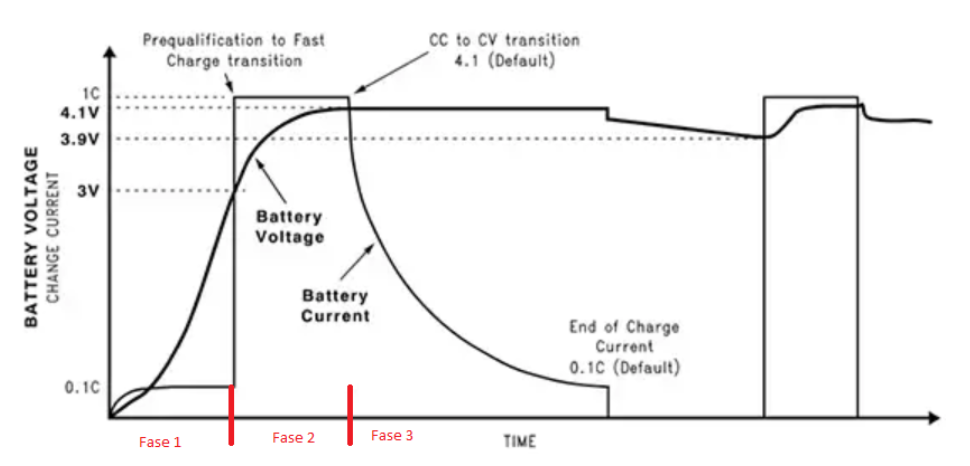
\includegraphics[scale=0.6]{figura/bateria/grafico.png}
\caption{Etapas de carga de bater�as Li-ion para una bater�a de 4.2[V]}
\label{grafico}
\end{figure}

Como se puede observar en la figura \ref{grafico}, la fase 1 ser�a la pre-condici�n de carga del 10\% por un tiempo determinado, luego entra a la fase 2 de corriente al m�ximo constante y finalmente pasa a la fase 3 donde se mantiene un voltaje constante mientras cae la corriente hasta que termina la carga. 
Cabe destacar que las corrientes se miden en t�rminos de la variable ``C`` la cual se refiere a la corriente que provee la bater�a, por ejemplo, una bater�a de $950[mA]$ posee un $C=950$. Esto es importante definir para poder realizar los c�lculos de las distintas etapas en el proceso de carga.
\section{Cargador de bater�a con corriente compartida con carga}
En la actualidad, todos los dispositivos electr�nicos tienden a ser lo mas simple posible, es por esto que los dise�os que se usan ahora poseen una bater�a interna que no se puede cambiar o no se deban sacar para cargarlas y as� facilitar la tarea al usuario. \\
Esto puede causar un problema debido a la pre-condici�n que existe en la fase 1 de la figura \ref{grafico}. Si el sistema empieza a pedir mucha corriente implicar�a que pueda que no se cumpla esa condici�n y en ese caso la carga (Arduino) estar�a descargando la bater�a en vez de permitir que se cargue, es por esto que existen integrados que pueden otorgar funcionamiento que permite la interacci�n de estos.\\
\section{MCP73871}
Considerando un integrado de microchip, el MCP73871\cite{bateria} otorga una funcionalidad de dise�ar un sistema que se encargue de cargar una bater�a de Li-ion con un sistema conectado, que en este caso ser�a el Arduino. En la tabla \ref{pinesmcp} se muestra la descripci�n de los pines que se utilizar�n en el dise�o.\\

\begin{table}[H]
\centering
\begin{tabular}{| c | c | c |}
\hline
\multicolumn{1}{|c|}{\textbf{N� Pin}}&
\multicolumn{1}{c|}{\textbf{Nombre}}&
\multicolumn{1}{|c|}{\textbf{Funci�n}}\\ \hline
1, 20 & Out & Salida hacia la carga\\ \hline
18, 19 & In & Entrada alimentaci�n\\ \hline
13 & PROG1 & Regulaci�n de corriente de carga r�pida\\ \hline
3 & SEL & Selecci�n de input\\ \hline
4 & PROG2 & L�mite de corriente entrada USB\\ \hline
12 & PROG3 & Corriente de t�rmino de la carga\\ \hline
14, 15 & VBAT & Conexi�n positiva con la bater�a\\ \hline
16 & VBAT\_ SENSE & Sensor de voltaje de la bater�a\\ \hline
\end{tabular}
\caption{Descripci�n de pines MCP73871}
\label{pinesmcp}
\end{table}

\subsection{Power Supply Input (IN)}
Este viene a ser la conexi�n a la alimentaci�n en la cual se puede usar un adaptador a la pared USB adem�s de poder cargarlo con un computador. Cuando se usa con la pared se debe considerar que el rango de voltaje debe estar entre $V_{bat} +300[mV]$ y $6[V]$. En este caso no habr�a problema ya que esta conexi�n USB provee $5[V]$ y la bater�a que se va a utilizar es de $3.6 [V]$.

\subsection{Input Source Type Selection (SEL)}
Este pin cumple una funci�n de selecci�n para carga r�pida. Con una entrada l�gica baja, el limite de carga es de baja corriente $100[mA]$, en cambio al utilizar una entrada l�gica alta, la entrada de corriente llega a ser de $500[mA]$. Este pin tiene una relaci�n con la selecci�n del nivel l�gico que tenga el pin ''SEL'' como se puede observar en la figura \ref{cargarapida}.\\
\begin{figure}[H]
\centering
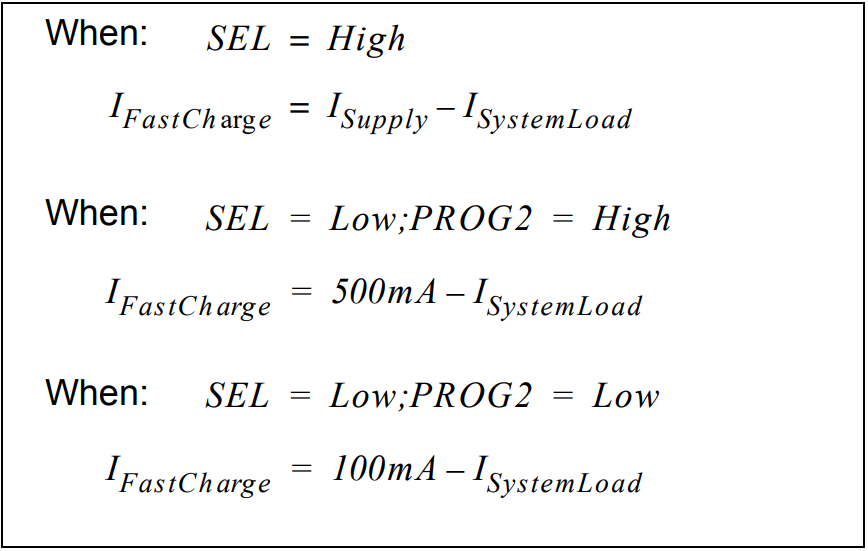
\includegraphics[scale=0.5]{figura/bateria/cargarapida.png}
\caption{Configuraciones disponibles para carga r�pida}
\label{cargarapida}
\end{figure}

Como se puede observar al utilizar ''SEL'' conectado a tierra permite que ''PROG2'' pueda ser utilizado cargando a $500[mA]$ o $100[mA]$ por lo que se elegir� la entrada de ''PROG2'' en alto para que se permita de igual manera cargar r�pido y utilizar todas las funciones del dispositivo dejando un l�mite de seguridad de $500[mA]$.

\subsection{Regulaci�n de carga r�pida(PROG1)}
El pin ''PROG1'' determina el m�ximo constante de corriente con un resistor entre el pin 13 y tierra. Este adem�s fija el m�ximo de corriente permitida y la corriente de t�rmino. Para calcular se debe considerar la ecuaci�n \ref{ivsR}.

\begin{equation}\label{ivsR}
I_{carga} = \frac{1000[V]}{R_{PROG1}[k\Omega]}
\end{equation}

Primero se debe conocer la corriente de carga $I_{Carga}$, para esto se utiliza la ecuaci�n  \ref{calculoRPROG}.
\begin{equation}\label{calculoRPROG}
R_{PROG1} = \frac{1000[V]}{I_{carga}} = 1.315[k\Omega] \approx 1.3[k\Omega]
\end{equation}

Despejando esta ecuaci�n se obtiene un resultado aproximado de $1.3[k\Omega]$ que ser� la resistencia utilizada para el dise�o

\subsection{Corriente de t�rmino de carga (PROG3)}

El ciclo de carga es terminado cuando, durante una etapa de voltaje constante (Figura \ref{grafico}), el promedio de corriente disminuye un l�mite (generalmente 0.1C) que se fija con un resistor conectado desde el pin ''PROG3'' hasta $V_{ss}$ el cual puede ser conectado a tierra.

\begin{equation}\label{Rprog3}
R_{PROG3} = \frac{1000[V]}{I_{Termino}} = 10.5[k\Omega] \approx 10[k\Omega]
\end{equation}

\subsection{Salida de voltaje a la bater�a $V_{BAT}$ y sensor de voltaje de bater�a $V_{SENSE}$}

Al conectar el terminal positivo de la bater�a de Li-ion el pin  $V_{BAT}$ cumple la funci�n de cargarla, es recomendable utilizar un capacitor de cer�mico en la salida para que asegure la estabilidad de la carga. 
El pin $V_{SENSE}$ se encarga de entregar el voltaje de salida para que el integrado se pueda realimentar con el valor que est� entregando y corregirlo. 

\subsection{Pines Generales}

Los pines mencionados anteriormente son los m�s relevantes con respecto a dise�o del dispositivo, hay otros pines que recomienda el fabricante utilizar como referencia para el usuario o el desarrollador los cuales muestran, conectando diodos led, Estado de bater�a, estado de carga y si se est� entregando o no alimentaci�n al dispositivo. 
Adem�s hay otras funciones que no se utilizan por lo que esos pines son conectados a tierra o al voltaje de alimentaci�n seg�n se especifique.

\subsection{Dise�o del esquem�tico}

Con todos los c�lculos anteriores, finalmente se dise�a el circuito con el integrado en el programa EagleCAD que ser� usado para enviar a producci�n de la PCB como se muestra en la figura \ref{esquematico22}.

\begin{figure}[H]
\centering
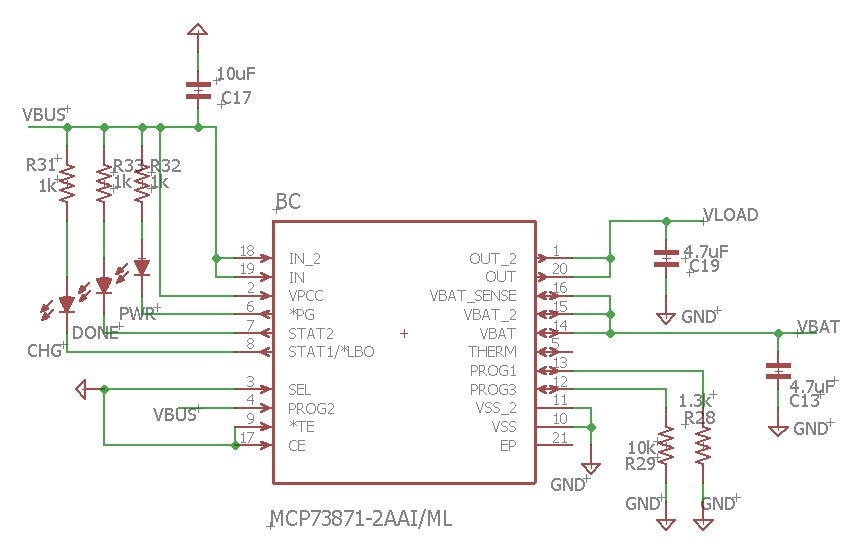
\includegraphics[scale=0.7]{figura/bateria/esquematico.jpg}
\caption{Dise�o de cargador de bater�a en software EagleCAD}
\label{esquematico22}
\end{figure}

Se puede observar los valores dise�ados para una bater�a de $3.7[V]$ de Li-ion con $950[mAh]$ de capacidad. Como se recomend� en $V_{BAT}$ es necesario utilizar condensadores de cer�mica para regular las salidas, al igual que en $V_{LOAD}$ el cual viene a ser el que se entrega al Arduino.\\
Se eligen los valores de ''SEL'' en $0[V]$ y ''PROG2'' en $5[V]$ para as� limitar la corriente de carga a la diferencia entre $500[mA]$ y la corriente de la carga, tal como se indica en la figura \ref{cargarapida}.

\newpage
\chapter{Dise�o final}\label{chap7}
En este capitulo se van a juntar las partes dise�adas anteriormente para obtener un esquem�tico final que ser� adaptado a una PCB utilizando el programa EagleCAD. Adem�s se dise�ar� un bot�n ON/OFF con el objetivo de no utilizar interruptores de 2 o mas posiciones.
\section{Bot�n ON/OFF}
Con las nuevas tecnolog�as van quedando obsoletos los botones o interruptores de 2 posiciones como se puede observar un ejemplo en la figura \ref{toggle} y tambi�n causado por la disminuci�n del tama�o de los dispositivos electr�nicos. 

\begin{figure}[H]
\centering
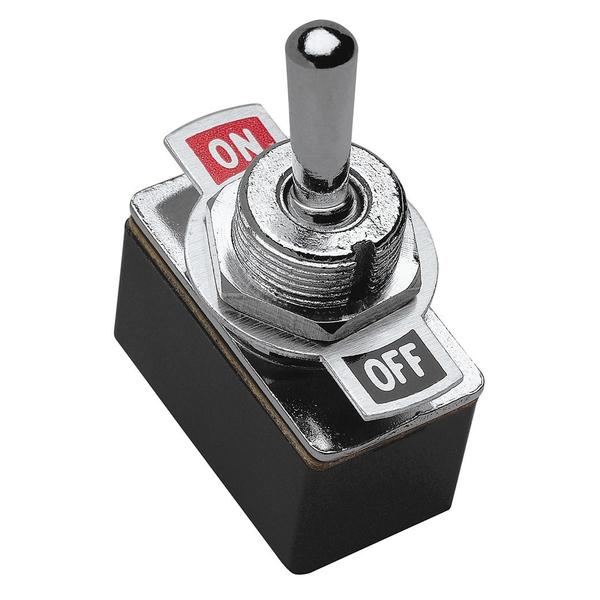
\includegraphics[scale=0.15]{figuras/eagle/toggle.png}
\caption{Interruptor de 2 posiciones}
\label{toggle}
\end{figure}

Estos interruptores ofrecen la funcionalidad que se necesita para un prototipo pero es necesario dise�ar un dispositivo final para entregar al cliente. Es por esto nace el requerimiento de que se deba usar un bot�n �nico para encender y apagar el dispositivo y esto no es una tarea trivial.\\
	Los requerimientos para este bot�n es que baje a $0[V]$ cuando se apaga, que sea un �nico bot�n y que no requiere ninguna programaci�n. \\

Un circuito muy utilizado que cumple los requerimientos anteriores se puede observar en la figura \ref{esquematico}.\\

\begin{figure}[H]
\centering
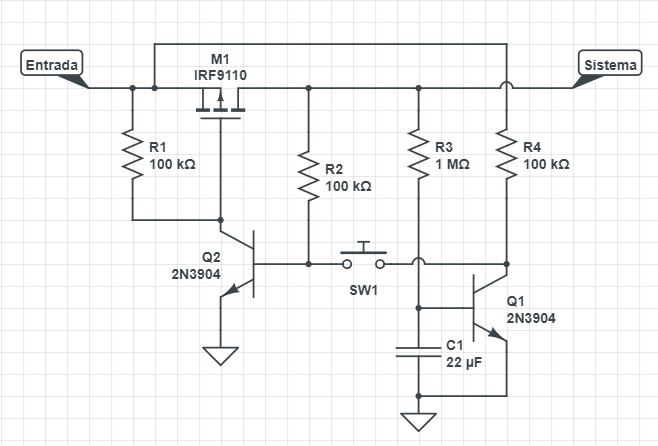
\includegraphics[scale=0.7]{figuras/eagle/circuito.png}
\caption{Circuito para bot�n ON/OFF}
\label{esquematico}
\end{figure}

Este circuito cumple con los requerimientos de ser simple, funcionar con un solo bot�n que cumple ambas funciones de encendido y apagado. \\
Alimentando el circuito con una entrada de $3[V]$ cuando se presiona el bot�n para encender, se alimenta la base del transistor Q2 lo que provoca que el mosfet M1 permita el paso de la corriente desde ''Drain'' hasta ''Source'' esto va a permitir que se alimente el sistema, adem�s va a alimentar el transistor Q1 lo que va a permitir cargar el condensador C1.\\
El condensador C1 es utilizado para mantener alimentado el transistor Q1 ya que al presionar el bot�n, una persona normal podr�a demorar entre $0.1[s]$ a $0.5[s]$ en todo el proceso ya que es humano, por lo que se utiliza para cargarlo en ese tiempo y no se apague autom�ticamente al soltar el bot�n.\\
En una segunda etapa cuando se pulsa el bot�n para apagar, se corta la base del transistor Q2 y utilizando la resistencia equivalente del Arduino el condensador se va a descargar pasando la corriente hacia el sistema y finalmente se cortar� la alimentaci�n.\\
Probando este circuito con un osciloscopio se puede corroborar el funcionamiento de encendido y apagado como se muestra en la figura  \ref{on}

\begin{figure}[H]
\centering
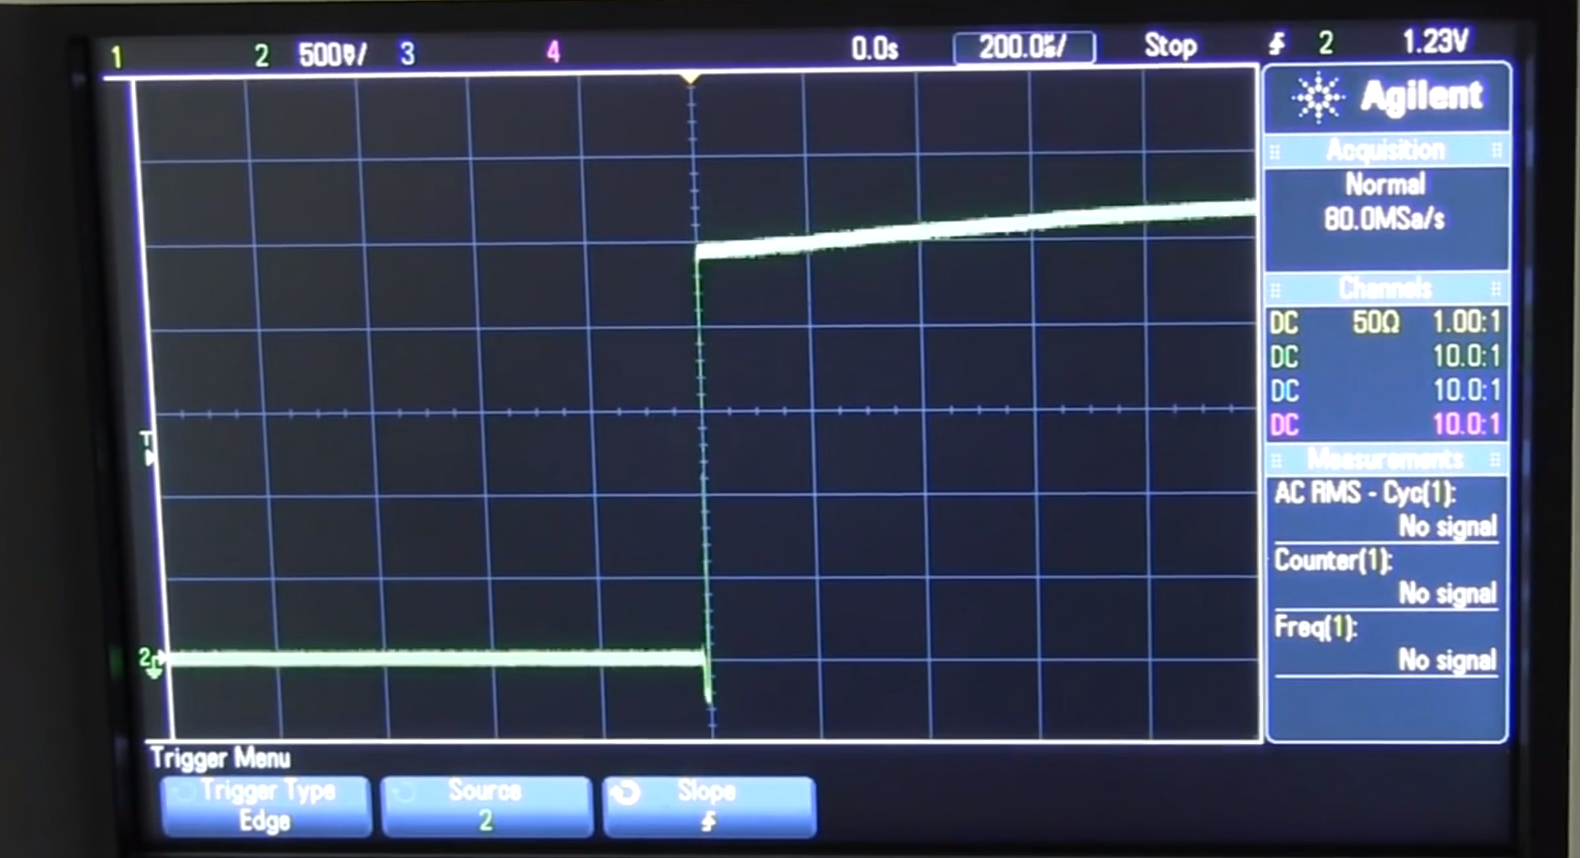
\includegraphics[scale=0.23]{figuras/eagle/on.png}
\caption{Funci�n de encendido}
\label{on}
\end{figure}

Esto muestra lo poco que demora el circuito en pasar de un estado a otro y permite mantenerse encendido.

\begin{figure}[H]
\centering
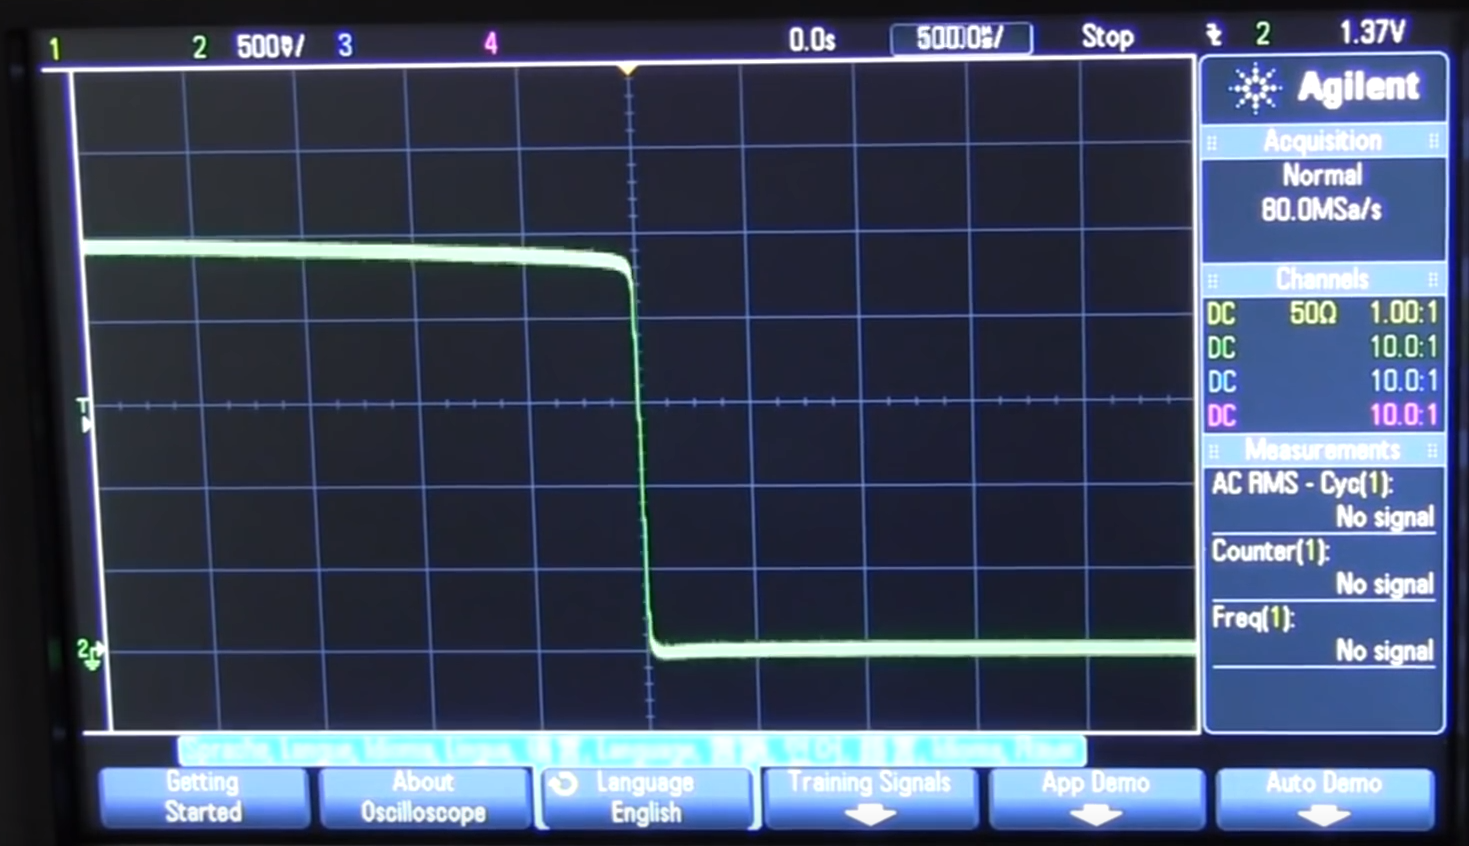
\includegraphics[scale=0.23]{figuras/eagle/off.png}
\caption{Funci�n de apagado}
\label{off}
\end{figure}

En la figura \ref{off} se puede observar que tambi�n se demora poco tiempo en descargarse, debido a que est� conectado a una carga muy grande y que pide mucha corriente, lo que hace que el tiempo de descarga del condensador C1 sea mucho menor. 

\section{Esquem�tico}
El dise�o final dispositivo se puede considerar como 7 m�dulos en conjunto entre los cuales se encuentra el microcontrolador, ECG, cargador de bater�a, bot�n ON/OFF, FTDI, Bluetooth y regulador de voltaje los cuales resultan en un esquem�tico final que se puede observar en los anexos.\\
Los m�dulos mas grandes se explicaron en los cap�tulos anteriores, en esta secci�n se explicar� el regulador de voltaje y los dise�os finales para el dispositivo.
\subsection{Regulador de voltaje 3.3[V]}
Para proveer energ�a al microcontrolador y al sistema entero, es necesario un regulador de voltaje de bajo ruido que cumpla la funci�n de evitar grandes variaciones que pueden provocar fallas en la PCB.\\
Todos los integrados utilizados tienen un rango aceptable de funcionamiento que var�a entre los $2-5[V]$ aproximadamente. En este intervalo los valores com�nmente utilizados son $3.3[V]$ y $5[V]$.\\
La alimentaci�n es un factor determinante a la hora de dise�ar un microcontrolador ya que al utilizar un resonador para sincronizar su reloj, dependiendo del voltaje que se provee, este funciona a distintas velocidades como se puede observar en la figura \ref{atmega}.\\

\begin{figure}[H]
\centering
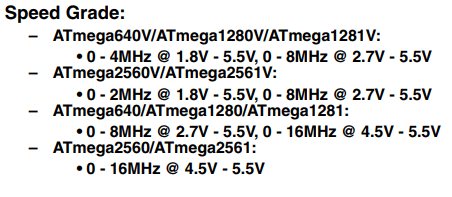
\includegraphics[scale=0.7]{figuras/eagle/atmega.png}
\caption{Velocidades y voltajes recomendados para un microcontrolador ATMega2560}
\label{atmega}
\end{figure}

Como se puede observar, es posible configurar el microcontrolador de $2[MHz]$ con voltaje entre $1.8[V]$ y $5.5[V]$. Adem�s una velocidad de $8[MHz]$ se puede conseguir con un voltaje entre $2.7$ y $5.5[V]$. Finalmente se puede utilizar una velocidad de $16[MHz]$ con un voltaje entre $4.5[V]$ y $5.5[V]$.\\
Como una de las condiciones es que el dispositivo sea de peque�o tama�o y peso, se utilizar� una bater�a de $4.3[V]$ de $950[mAh]$ y es por esto que se va a bajar la velocidad a $8[MHz]$ para utilizar una alimentaci�n de $3.3[V]$.\\

Se utilizar� un integrado MIC5219 el cual ofrece un regulador de bajo ruido que funciona a $3.3[V]$ y permitir� energizar el dispositivo. En la figura \ref{reg} se puede observar el integrado y su configuraci�n t�pica.

\begin{figure}[H]
\centering
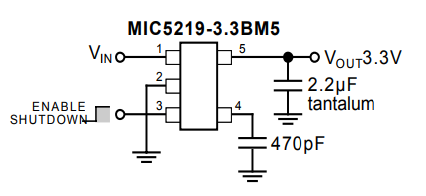
\includegraphics[scale=1]{figuras/eagle/reg.png}
\caption{Regulador de voltaje 3.3[V]}
\label{reg}
\end{figure}

Para entender este diagrama es necesario destacar $V_{in}$ que viene a ser la alimentaci�n de la bater�a de Li-ion, $V_{out}$ es la salida de $3.3[V]$ hacia la carga que involucra el microcontrolador y todas las componentes del sistema.\\
El pin 2 es la tierra del sistema y el pin 3 ofrece una funci�n para habilitar y deshabilitar el regulador la cual no se va a utilizar. Finalmente el pin 4 ofrece reducci�n de ruido conectandolo a tierra con un condensador de $470[pF]$.

\subsection{Conector para sensores}
Al trabajar con sensores, es necesario facilitar la tarea para el dise�ador de producto de conectar las entradas al sistema con el vestible, es por esto que se va a reducir todos los sensores a un solo conector. Para esto, considerando que se utilizar� el ECG y 2 sensores de temperatura para promediar su valor y obtener mayor precisi�n, se necesitan 5 conectores para los datos y adem�s alimentaci�n y tierra.\\

\begin{figure}[H]
\centering
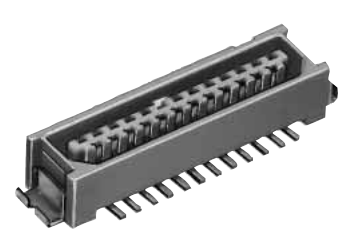
\includegraphics[scale=0.5]{figuras/eagle/conn.png}
\caption{Conector para sensores}
\label{conector}
\end{figure}

El conector que se utilizar� se puede observar en la figura \ref{conector}. La particularidad que ofrecen estos tipos de conectores es que poseen entre 9 y 51 contactos.\\
Para el dise�o se van utilizar 9 contactos los cuales constan de 3 conectores para los 3 electrodos de ECG, 2 para sensores de temperatura y 4 de alimentaci�n (Voltaje y tierra para ECG independientes de la alimentaci�n de los sensores de temperatura) como se puede observar en la figura \ref{coneagle}.

\begin{figure}[H]
\centering
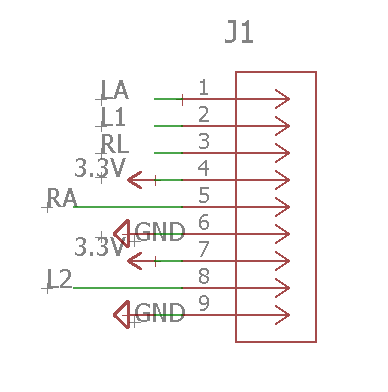
\includegraphics[scale=0.5]{figuras/eagle/sensores.png}
\caption{Conector de 9 pines}
\label{coneagle}
\end{figure}

\subsection{Pin header para prototipo}
Finalmente, como el microcontrolador ofrece 16 pines an�logos, 54 digitales y 14 PWM se dejar�n headers en la primera iteraci�n del dispositivo para que se pueda seguir prototipando y agregar mas sensores en el futuro, donde se pueda trabajar en el mismo dispositivo en vez de utilizar uno independiente. \\
Tambi�n se va a dejar disponible pines para comunicaci�n UART (2 utilizadas en el dispositivo y 2 libres) y tambi�n los pines SDA y SCL para comunicaci�n I2C. \\

\begin{figure}[H]
\centering
\includegraphics[scale=0.5]{figuras/eagle/header.png}
\caption{Conecci�n Headers}
\label{header}
\end{figure}

Como se puede notar en la figura \ref{header} estos pines ofreceran alimentaci�n y comunicaci�n UART en cada header. 3 pines analogos (A3, A4 y A5), los 2 pines de conecci�n I2C (SDA y SCL) y 5 pines digitales (PA0, PA1, PA2, PB4 y PB5).







\newpage
\chapter{Discusi�n}\label{chap11}

Este trabajo tuvo el prop�sito de buscar una soluci�n al desaf�o propuesto por la empresa Sistemas Expertos. Como grupo multidisciplinario se tom� la decisi�n de no dejar el trabajo e investigaci�n realizada solo como un prototipo por lo que se llev� al �rea del emprendimiento postulando a fondos para desarrollar mejor la idea y proponer el modelo de negocios desarrollado durante el a�o.

\section{Transformaci�n de memoria multidisciplinaria a emprendimiento}
Al finalizar el dise�o del dispositivo y tener un prototipo funcional como grupo de memorias multidisciplinarias se decidi� continuar trabajando en el desaf�o con una alianza estrat�gica con la empresa Sistemas Expertos.\\
Se realizaron entrevistas con profesionales de la salud en el �rea de Quintero y se postul� a un torneo de emprendimiento del instituto 3IE de la universidad Santa Mar�a.\\
El Instituto 3IE tiene como principal objetivo apoyar el desarrollo y aceleraci�n de emprendimientos de base tecnol�gica, con m�rito innovador y alto potencial de escalamiento, a trav�s de su Programa de Incubaci�n, cuya principal propuesta de valor se basa en vinculaci�n temprana con el sector productivo o empresarial, la validaci�n t�cnico y comercial de las soluciones (productos y/o servicios), la gesti�n comercial, y el financiamiento temprano para hacer despegar los negocios.\\
Este Programa, se implementa bajo la l�nea de financiamiento Torneos de Emprendimiento Tecnol�gico, apoyado por CORFO y ejecutado por el Instituto 3IE, y que busca instalar capacidades y conocimientos en tecnolog�as habilitantes para el desarrollo de nuevas soluciones tecnol�gicas que logren un impacto positivo en la competitividad y eficiencia del sector industrial o p�blico.\\

\begin{figure}[H]
\centering
\includegraphics[scale=0.3]{figuras/chamullo/corfo.jpg}
\caption{Desaf�o IoT propuesto por el instituto 3IE}
\label{3ie}
\end{figure}

\newpage
Este concurso posee una planificaci�n del proceso completo que se puede observar en la figura \ref{proceso}

\begin{figure}[H]
\centering
\includegraphics[scale=0.85]{figuras/chamullo/proceso.jpg}
\caption{Planificaci�n desaf�o IoT}
\label{proceso}
\end{figure}


\subsection{Entrevista a doctores en hospital de Quintero}
Se realizaron entrevistas a 2 profesionales de la salud en el hospital de quintero para evaluar la factibilidad del emprendimiento y ver el problema desde el punto de vista de quienes trabajan en el sector p�blico.\\
Primero se realiz� la entrevista a Fabi�n �lvarez, medico general de zona y cuyo cargo es jefe de urgencia. Tambi�n se realiz� una entrevista al doctor Cristian Mondaca, Jefe del programa de salud cardiovascular y jefe de farmacia. 
\subsubsection{Entrevista a Fabi�n �lvarez}
En la entrevista comenta que los adultos sanos realizan controles 1 vez al a�o y se hacen ex�menes preventivos. Adem�s existe un programa de salud cardiovascular para personas mayores de 18 a�os, seg�n gu�as cl�nicas "Enfoque de riesgo cardiovascular" del MINSAL (2015), cada 3, 6 y 12 meses en los cuales se hacen ex�menes de laboratorio, electrocardiograma, se mide presi�n arterial, peso y estatura. 
Los problemas que se identificaron fueron la poca disponibilidad de ex�menes y recursos humanos para atender a la demanda programada. Adem�s implementan telemedicina por medio de fotos para dermatolog�a donde le env�an estas a alg�n especialista, teleasistencia broncopulmonar mediante videoconferencia y teleasistencia para electrocardiograma el cual intenta no usarse demasiado.\\
Debido a la sobre demanda del sistema de urgencias, los profesionales de la salud deciden hacer una categorizaci�n de pacientes desde C1 a C5 donde C5 significa que requiere asistencia inmediata y C1 puede ser que el paciente vuelva otro d�a.\\
Finalmente se hizo una encuesta donde el m�dico deb�a dar un valor a las siguientes afirmaciones seg�n un ranking de dolor entre 1 y 10 como se muestra en la tabla \ref{fabian}
\newpage
\begin{table}[H]
\centering
\begin{tabular}{| c | c |}
\hline
\multicolumn{1}{|c|}{\textbf{Afirmaci�n}}&
\multicolumn{1}{|c|}{\textbf{Nota de Dolor}}\\ \hline
Muchos Recursos por IIH  & 3-4  \\ \hline
Necesidad de control mas r�pido en urgencias & 8 \\ \hline
Reclamo por el servicio  & 10  \\ \hline
Reclamos internos de los m�dicos & 10\\ \hline
Bajos recursos para mejorar atenci�n & 10\\ \hline
\end{tabular}
\caption{Ranking de dolor Fabi�n �lvarez}
\label{fabian}
\end{table}

\subsubsection{Entrevista a Cristian Mondaca}
Como jefe del programa de salud cardiovascular, da �nfasis en el riesgo cardiovascular con controles cada 3, 6 y 12 meses y destaca que muchas veces se atrasa a los pacientes que van mejorando pese a que no se deber�a hacer debido a la disponibilidad de horas m�dicas y la cantidad de pacientes.
En caso de mayor necesidad se tiene contemplado el uso de una hora extra al mes siguiente por ex�menes nuevos.\\
Se mostr� un v�deo con el prototipo funcional realizado en este trabajo de tesis y el m�dico hace la observaci�n de que para realizar controles se requiere hacer un ECG completo, es decir, se necesitan las 6 precordiales y las 3 tradicionales (2 electrodos en brazos y 1 en pierna). \\
En la entrevista destaca que para realizar pruebas en pacientes reales se debe hablar con el director del hospital y desarrollar un consentimiento informado de parte del paciente. \\
Un dato importante que resalta es la cantidad de pacientes en el programa de salud cardiovascular el cual alcanza un total de 1900 incluyendo hipertiroidismo, de los cuales 1500 son de mayor riesgo.\\
Entre las ideas propuestas por el m�dico se destaca la necesidad de tener una base de datos con historial de electrocardiogramas ya que al realizar ex�menes tradicionales estos se imprimen en un papel milim�trico y son otorgados a los pacientes, los cuales generalmente pierden esta informaci�n para la pr�xima consulta lo que hace m�s dif�cil un diagnostico preciso.\\
Finalmente se hace �nfasis en que el hospital de Quintero es un hospital de baja complejidad y no hay especialistas, por lo que cuando hay alguna anormalidad se deriva a un cardi�logo o medico internista para realizar un informe y diagnosticar.\\
Cuando ocurre un infarto, es enviado en ambulancia directo a Vi�a del mar para que sea atendido por un especialista.

\subsection{Pitch day selecconados - Marzo 2018}
Para realizar el Pitch para el concurso se utiliz� lo aprendido en los m�dulos de memoria y las clases impartidas por el desaf�o del instituto 3IE en los cuales dividen el pitch en 3 partes.\\
La primera parte es hablar del dolor, identificar cuantos tipos de cliente se ven afectados y mostrarlos en t�rminos objetivos (cifras), con esto se debe presentar cuales son los analg�sicos internos, externos y como se evitan este dolor y finalmente presentar una promesa de valor en la cual se explica, de manera simple, que logra nuestra soluci�n. Para esto se recopil� informaci�n y se identific� que solo para el a�o 2016 fallecieron alrededor de $25.000$ personas esperando atenci�n m�dica en alguno de los 203 hospitales p�blicos chilenos. De esos, $18.423$ ( $74\%$ aproximadamente) corresponden a personas sobre 65 a�os. Esto solo refleja un universo mucho mayor, cercano a $1.661.826$ de personas que estuvieron en lista de espera y la �nica forma de mitigar esto es por medio de categorizaci�n de pacientes por su nivel de riesgo, lo cual no disminuye las listas, sino que da prioridad a aquellos mas urgentes\\
La segunda parte consiste en el servicio propiamente tal, donde se plantea reducir las listas de espera y tener una gesti�n eficiente del capital humano donde los profesionales atienden donde y a quien corresponde en base a un historial. Proyecto Galeno ofrece una polera inteligente con sensores de electrocardiograma y temperatura conectada a un dispositivo Android que a su vez env�a la informaci�n a un sitio web donde muestra en tiempo real la informaci�n y donde tambi�n se puede controlar el comportamiento del ecosistema.\\
En la tercera parte se muestra el plan de vuelo donde se dan a conocer los hitos relevantes del proyecto, el plan de negocio y el equipo. La obtenci�n de dinero es posible a trav�s de un sistema de arriendo mensual de los dispositivos y la plataforma en cada hospital, seg�n las necesidades de cada uno. Como en caso concreto se tiene al Hospital de Quintero con alrededor de 34 camas disponibles y un ejemplo de pacientes con patolog�as cardiovasculares, pudiendo proyectar al menos entre $2000$ y $6000$ USD mensuales (considerando entre 10 y 30 dispositivos a $200$ USD cada uno).\\
Finalmente se cierra presentando el equipo y presentando nuestro aliado estrat�gico Sistemas Expertos, empresa que posee presencia en el mercado de la atenci�n p�blica con 17 centros asistenciales a lo largo de Chile en el servicio de software para digitalizaci�n de la informaci�n.\\
En esta fase concluye la participaci�n de Proyecto Galeno en el desaf�o IoT debido a que el jurado considera que la inversi�n en el desarrollo y la validaci�n del dispositivo para obtener la certificaci�n de grado m�dico es muy grande, se propone abordar este mismo problema externalizando el desarrollo con un dispositivo que ya tenga validaci�n m�dica buscando aliados estrat�gicos para poder desarrollar a partir de esto. Adem�s la presencia de Accuhealth en el mercado ofrece el mismo servicio con una mayor gama de sensores a un precio un poco superior al calculado por este proyecto, lo que hace muy dif�cil entrar al mercado de la salud privada y no consideran que entrar en el sistema de salud p�blico sea una buena oportunidad.
\newpage
\section{Tareas Futuras}

La primera versi�n de un dispositivo electr�nico es solo el comienzo de un largo camino en el desarrollo ya que es donde se puede evaluar de mejor manera el funcionamiento del dise�o y evaluar cuales son los puntos a mejorar o cambiar. \\
En primera instancia se desea integrar la IMU en la siguiente iteraci�n utilizando los headers de comunicaci�n I2C que se dise�aron para prototipado y evaluar la posibilidad de cambiar el integrado amplificador para la se�al del ECG a uno con menor ruido y mayor precisi�n. \\
Adem�s se dise�� un modulo de bot�n ON/OFF y cargador de bater�a de forma independiente, lo cual se puede sustituir por un solo integrado lo cual disminuir�a mucho el tama�o, pero esta idea fue descartada para la primera versi�n debido a que aumenta mucho el costo de fabricaci�n debido a su empaquetado lo cual requiere un servicio adicional para soldarlo en la PCB final.\\


\newpage
% ---------------------------------------------------------------------------------------
\chapter{Conclusiones}\label{chap9}
Al ver el esquem�tico terminado y las piezas seleccionadas se puede notar que se cumplen los requisitos propuestos en un principio. Realizando un listado de costos de componentes se obtiene un valor de $42 USD$ total. Adem�s el costo de fabricaci�n de una PCB de tama�o menor a $10x10[cms]$ es de aproximadamente $7 USD$. Lo que lleva a un costo total del dispositivo de $49 USD$ contando solamente componentes electr�nicas.\\
Es importante destacar que esta primera versi�n del dispositivo es solo un comienzo en la larga etapa de desarrollo, luego de producir esta primera placa se debe realizar las pruebas correspondientes y verificaci�n de integridad de la placa.\\
El dise�o final de la PCB se puede observar en los anexos.\\
Adem�s se aprendi� a dise�ar un dispositivo electr�nico desde su prototipo en una placa de desarrollo, donde fue necesario leer constantemente las hojas de datos de todas las componentes a utilizar y seleccionar cuales son las mejores, que al mismo tiempo sean compatibles y coherente con el dise�o que se est� llevando a cabo.\\
Tambi�n es importante destacar la experiencia que se obtuvo con el concurso de emprendimiento. Se aprendi� mucho del mundo del emprendimiento al presentar el trabajo realizado. Adem�s se tuvo la oportunidad de observar los trabajos propuestos por los otros emprendedores y estudiar los criterios de evaluaci�n. Se di� mucha importancia al modelo de negocios y las alianzas estrat�gicas que ten�a cada participante, mas que al trabajo realizado y estado actual de la idea o prototipo. Muchos de los seleccionados ya ten�an potenciales clientes y alianzas estrat�gicas que los hac�a mejores candidatos a ganar el dinero para el emprendimiento.

\newpage
% ---------------------------------------------------------------------------------------
\chapter{Anexos}\label{Anexos}
%\newpage
\includepdf[pages={-},scale=0.9,pagecommand={}]{figura/anexos/esquematic.pdf}
\includepdf[pages={-},scale=1.1,pagecommand={}]{figura/anexos/board.pdf}
\includegraphics[width=1\textwidth]{figura/anexos/code1.jpg}
\includegraphics[width=1\textwidth]{figura/anexos/code2.jpg}
\includegraphics[width=1\textwidth]{figura/anexos/code3.jpg}
\includegraphics[width=1\textwidth]{figura/anexos/code4.jpg}
\includegraphics[width=1\textwidth]{figura/anexos/code5.jpg}
\includegraphics[width=1\textwidth]{figura/anexos/code6.jpg}
\includegraphics[width=1\textwidth]{figura/anexos/code7.jpg}
\includegraphics[width=1\textwidth]{figura/anexos/code8.jpg}
\includegraphics[width=1\textwidth]{figura/anexos/code9.jpg}
\centering
\includegraphics[width=1\textwidth]{figura/anexos/code10.jpg}


\newpage
\renewcommand{\refname}{Referencias}
\begin{thebibliography}{99}

\bibitem{visi} Sotera Wireless, ViSi Mobile\textregistered  System, rev. 05 marzo 2018, \hyperref[visi]{http://www.soterawireless.com/visi-mobile/}

\bibitem{visi_tel} Sotera Wireless, ViSi Mobile\textregistered  System, rev. 15 Mayo 2018, \hyperref[visi_tel]{https://newatlas.com/visi-mobile-wireless-health-monitoring/25583/}

\bibitem{qardio} Qardio Inc., QardioCore, rev.  05 marzo 2018, \hyperref[qardio]{https://www.getqardio.com/es/qardiocore-wearable-ecg-ekg-monitor-iphone/}

\bibitem{qardio_tel} Qardio Inc., QardioCore, rev.  15 Mayo 2018,
\hyperref[qardio_tel]{https://store.getqardio.com/products/qardiocore}

\bibitem{nuubo} Nuubo, Nuubo wearable ECG, rev. 05 marzo 2018, \hyperref[nuubo]{https://www.nuubo.com/producto}

\bibitem{nuubo_tel} Nuubo, Nuubo wearable ECG, rev. 15 Mayo 2018, \hyperref[nuubo_tel]{http://pdf.medicalexpo.com/pdf/nuubo/necg-minder/83949-96239.html}

\bibitem{ad8232} Analog Devices, ``Single-Lead Heart Rate Monitor Front End'', Rev. B Marzo 2017, \hyperref[ad8232]{http://www.analog.com/media/en/technical-documentation/data-sheets/AD8232.pdf}

\bibitem{RN4020} Microchip, ``Bluetooth Low Energy Module RN4020'', Rev. 15 Mayo 2018, \hyperref[RN4020]{http://ww1.microchip.com/downloads/en/DeviceDoc/50002279B.pdf}

\bibitem{RF} Wikipedia, ``Radio Frecuencia'', Rev. 15 Mayo 2018, \hyperref[RF]{https://es.wikipedia.org/wiki/Radiofrecuencia}

\bibitem{satelite} Wikipedia, ``Comunicaciones por satélite'', Rev. 15 Mayo 2018, \hyperref[satelite]{https://goo.gl/ykf7tv}

\bibitem{wifi} Wikipedia, ``IEEE 802.11'', Rev. 15 Mayo 2018, \hyperref[wifi]{https://goo.gl/1hmiWW}

\bibitem{celular} Wikipedia, ``Red de celdas'', Rev. 15 Mayo 2018, \hyperref[celular]{https://goo.gl/K2sKoQs}

\bibitem{temp} Maxim Integrated, ``Programable Resolution 1-Wire Digital Thermometer'', rev Enero 2015, \hyperref[temp]{https://datasheets.maximintegrated.com/en/ds/DS18B20.pdf}

\bibitem{xbee_info} XBee, ``¿Qué es XBee?'', rev Mayo 2018, \hyperref[xbee_info]{http://xbee.cl/que-es-xbee/}

\bibitem{AT} Wikipedia, ``Conjunto de comandos Hayes'', rev Mayo 2018, \hyperref[AT]{https://goo.gl/xpCfKC}

\bibitem{ecg_rate} Fire EMS, ``Understanding ECG Filtering'', rev Mayo 2018, \hyperref[ecg_rate]{http://www.ems12lead.com/2014/03/10/understanding-ecg-filtering/}

\bibitem{bluetooth} Wikipedia, ``Bluetooth'', rev Mayo 2018, \hyperref[bluetooth]{https://es.wikipedia.org/wiki/Bluetooth}

\bibitem{market_share_cita} StatCounter, ``GlobalStats'', rev Mayo 2018, \hyperref[market_share_cita]{https://goo.gl/62GngF}

\bibitem{hosting_web} Wikipedia, ``Alojamiento Web'', rev Mayo 2018, \hyperref[hosting_web]{https://es.wikipedia.org/wiki/Alojamiento\_web}

\bibitem{services} Google, ``Servicios'', rev Julio 2018, \hyperref[services]{https://developer.android.com/guide/components/services?hl=es-419}

\bibitem{RN4020_code} Microchip, ``RN4020'', rev Julio 2018, \hyperref[RN4020_code]{https://www.microchip.com/wwwproducts/en/RN4020}

\bibitem{realm_android} Realm, ``Realm Android'', rev Julio 2018, \hyperref[realm_android]{https://realm.io/blog/realm-for-android}

\bibitem{user_guide_rn4020} Microchip, ``RN4020 User Guide'', rev Julio 2018, \hyperref[user_guide_rn4020]{http://ww1.microchip.com/downloads/en/DeviceDoc/70005191B.pdf}

\bibitem{java8} Android, ``Usar funciones del lenguaje de Java 8'', rev Julio 2018, \hyperref[java8]{https://developer.android.com/guide/platform/j8-jack}

\bibitem{proguard} ProGuard, ``The open source optimizer for Java bytecode'', rev Julio 2018, \hyperref[prroguard]{https://www.guardsquare.com/en/products/proguard}

\bibitem{flutter} Flutter, ``Build beautiful native apps in record time'', rev Julio 2018, \hyperref[flutter]{https://flutter.io}

\bibitem{kotlin} Kotlin, ``Statically typed programming language for modern multiplatform applications'', rev Julio 2018, \hyperref[kotlin]{https://kotlinlang.org}


\bibitem{http2sse} InfoQ, ``Will WebSocket survive HTTP/2?'', rev Julio 2018, \hyperref[http2sse]{https://www.infoq.com/articles/websocket-and-http2-coexist}

\bibitem{unittest} Android Developers, ``Build effective unit tests'', rev Julio 2018, \hyperref[unittest]{https://developer.android.com/training/testing/unit-testing}

\bibitem{sonarqube} SonarQube, ``Continuous
Code Quality'', rev Julio 2018, \hyperref[sonarqube]{https://www.sonarqube.org}

\bibitem{tensor} TensorFlow, ``An open source machine learning framework for everyone'', rev Julio 2018, \hyperref[tensor]{https://www.tensorflow.org}


\bibitem{mxnet} SonarQube, ``A flexible and efficient library for deep learning'', rev Julio 2018, \hyperref[mxnet]{https://mxnet.apache.org}

\bibitem{jenkins} Jenkins, ``Build great things at any scale'', rev Julio 2018, \hyperref[jenkins]{https://jenkins.io}

\bibitem{nodejs} NodeJS, ``NodeJS'', rev Julio 2018, \hyperref[nodejs]{https://nodejs.org/es}

\bibitem{socket} Socket.io, ``FEATURING THE FASTEST AND MOST RELIABLE REAL-TIME ENGINE'', rev Julio 2018, \hyperref[socket]{https://socket.io/}

\bibitem{angularjs} AngularJS, ``AngularJS'', rev Julio 2018, \hyperref[angularjs]{https://angularjs.org/}

\bibitem{expressjs} ExpressJS, ``Infraestructura web rápida, minimalista y flexible para Node.js'', rev Julio 2018, \hyperref[expressjs]{http://expressjs.com/es/}

\bibitem{meteor} MeteorJS, ``THE FASTEST WAY TO BUILD JAVASCRIPT APPS'', rev Julio 2018, \hyperref[meteor]{https://www.meteor.com/}

\bibitem{mongoose} Mongoose, ``Elegant mongodb object modeling for node.js'', rev Julio 2018, \hyperref[mongoose]{http://mongoosejs.com/}

\bibitem{influxdb} InfluxDB, ``The modern engine for Metrics and Events'', rev Julio 2018, \hyperref[influxdb]{https://www.influxdata.com/}

\bibitem{firebase} FireBase, ``Firebase te ayuda a crear mejores apps para dispositivos móviles y hacer crecer tu empresa.'', rev Julio 2018, \hyperref[firebase]{https://firebase.google.com/?hl=es-419}

\bibitem{postgresql} PostgreSQL, ``THE WORLD'S MOST ADVANCED OPEN SOURCE RELATIONAL DATABASE'', rev Julio 2018, \hyperref[prostgresql]{https://www.postgresql.org/}

\bibitem{grafana} Grafana, ``The open platform for beautiful analytics and monitoring'', rev Julio 2018, \hyperref[grafana]{https://grafana.com/}

\bibitem{d3} D3, ``D3: Data-Driven Documents'', rev Julio 2018, \hyperref[d3]{https://d3js.org/}

\bibitem{highcharts} HighCharts, ``Make your data come alive'', rev Julio 2018, \hyperref[highcharts]{https://www.highcharts.com/}

\bibitem{chartjs} ChartJS, ``Simple yet flexible JavaScript charting for designers \& developers'', rev Julio 2018, \hyperref[chartjs]{https://www.chartjs.org/}

\bibitem{websocket} Wikipedia, ``WebSocket'', rev Julio 2018, \hyperref[websocket]{https://es.wikipedia.org/wiki/WebSocket}

\bibitem{namecheap} Namecheap, ``Search for your domain name'', rev Julio 2018, \hyperref[namecheap]{https://www.namecheap.com/}

\bibitem{atmosphere} Atmosphere, ``Explore Meteor Packages'', rev Julio 2018, \hyperref[atmosphere]{https://atmospherejs.com/}

\bibitem{ddp} Meteor, ``Server Connections'', rev Julio 2018, \hyperref[ddp]{https://docs.meteor.com/api/connections.html}

\bibitem{mongodb} MongoDB, ``MongoDB for GIANT Ideas'', rev Julio 2018, \hyperref[mongodb]{https://www.mongodb.com/}

\bibitem{nginx} NGINX, ``NGINX | High Performance Load Balancer, Web Server \& Reverse Proxy'', rev Julio 2018, \hyperref[nginx]{https://www.nginx.com/}

\bibitem{certbot} CertBot, ``Automatically enable HTTPS on your website with EFF's Certbot, deploying Let's Encrypt certificates.'', rev Julio 2018, \hyperref[certbot]{https://certbot.eff.org/}

\bibitem{nginx_certbot} SeaFile-docs, ``Enabling Https with Nginx'', rev Julio 2018, \hyperref[nginx_certbot]{https://manual.seafile.com/deploy/https\_with\_nginx.html}

\comm{



\bibitem{isp} Microchip, ``In-Circuit Serial Programming (ICSP) Guide'', rev Enero 2015, \hyperref[temp]{http://ww1.microchip.com/downloads/en/devicedoc/30277d.pdf}

\bibitem{ft232} FTDI Chip, ``Future Technology Devices International Ltd. FT232R USB UART IC'', rev 18 noviembre 2015, \hyperref[temp]{http://www.ftdichip.com/Support/Documents/DataSheets/ICs/DS\_ FT232R.pdf}

\bibitem{bateria} Microchip, ``Stand\- Alone System Load Sharing and Li\- Ion Baterry Charge Management Controller'', rev Septiembre 2013, \hyperref[temp]{http://ww1.microchip.com/downloads/en/DeviceDoc/20002090D.pdf}
}
%
%\bibitem{NETR/NETW} How is data exchanged between two SIMATIC S7-200 %devices in PPI mode?\\
%\hyperref[NETRNETW]{https://support.industry.siemens.com/cs/document/%370000/how-is-data-exchanged-between-two-simatic-s7-200-devices-in-ppi-%mode-?dti=0\&lc=en-WW} 
%
\end{thebibliography}

		
\end{document}